\documentclass{article}
\usepackage[T1]{fontenc}

\usepackage{graphicx}
\usepackage{parskip}
\usepackage{xcolor}
\usepackage[colorlinks=true,linkcolor=black]{hyperref}
\usepackage[french]{babel}
\usepackage{subcaption}
\usepackage[french]{babel}

\usepackage[margin=3.5cm]{geometry}


\author{Erwan LEMATTRE \and Yannis CHUPIN}
\title{Rapport\\Fairness pour l'IA}
\date{Avril 2024}

\begin{document}
    \maketitle
    \newpage
    \tableofcontents
    \newpage

    \section{Introduction}
    Ce projet a pour objectif d'analyser les accidents de la circulation routière afin de pouvoir déterminer 
    à partir des données d'un véhicule accidenté si l'accident est mortel ou non.
    Les données sont des données libres mises à disposition par le \textit{Ministère de l'Intérieur et des 
    Outre-Mer}. Le jeu de données correspond aux accidents de 2005 à 2022 en France. Nous allons, dans une première 
    partie, analyser ces données afin d'extraire les informations utiles à l'apprentissage. Puis nous essaierons de repérer 
    d'éventuelles sources de biais affectant notre modèle.
    
    Vous pouvez retrouver le code sur le GitHub du projet. Le fichier \texttt{main.ipynb} contient 
    le code principal que nous allons suivre et contextualiser tout au long de ce rapport. de plus, le fichier \texttt{utils.py} 
    contient toutes les fonctions auxiliaires que nous utilisons dans le fichier principal.

    \newpage
    \part{Analyse}
    \section{Découverte du jeu de données}
    \subsection{La base de données}
    La base de données est composée de plusieurs tables : \textit{usagers}, \textit{véhicules}, \textit{lieux} et 
    \textit{caractéristiques}. Nous avons joint ces quatre parties pour obtenir un dataframe contenant une 
    cinquantaine de colonnes. 
    On peut retrouver une partie des attributs dans l'annexe \ref{appendix:dataset}.


    \subsection{Répartition des données}
    Afin de pouvoir conserver les données utiles pour l'apprentissage, nous avons analysé la répartition des 
    différentes données dans notre dataframe.
    Nous avons ainsi pu faire différentes observations. 
    \\
    Voici quelques-unes d'entre elles qui nous sont ensuite utiles pour la préparation des données.
    \subsubsection{Catégories de véhicule}
    La base de données contient beaucoup de types de véhicules différents. Nous avons cependant pu remarquer 
    que la majorité des véhicules sont dans seulement 5 catégories.
    \begin{figure}[ht]
        \centering
        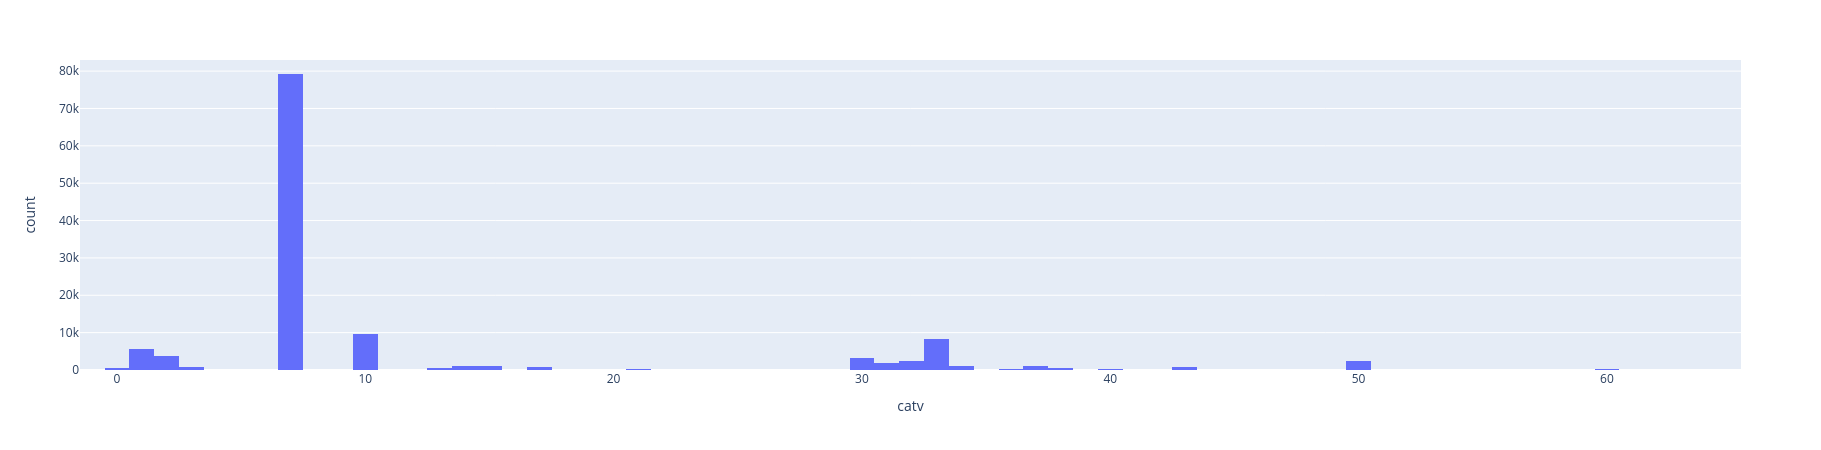
\includegraphics[width=12cm]{./img/catv1.png}
        \caption{Répartition des catégories de véhicules}
    \end{figure}

    \subsubsection{Gravité de l'accident}
    En affichant l'effectif d'individus décédés dans un accident, nous avons pu remarquer qu'ils ne représentent qu'une 
    infime partie des individus accidentés. Leur proportion est si fable que ça ne nous permet pas d'apprendre 
    un modèle. C'est la raison pour laquelle nous avons décidé de nous intéresser non pas à la mortalité 
    à l'échelle d'une personne, mais plutôt à l'échelle d'un accident. Nous nous mettons pour cela au niveau d'un 
    véhicule car cela nous permet de conserver plus d'informations (à l'échelle d'un accident, on aurait 
    dû enlever trop d'informations pour ne conserver que les attributs plus généraux à l'accident).

    \begin{figure}[ht]
        \centering
        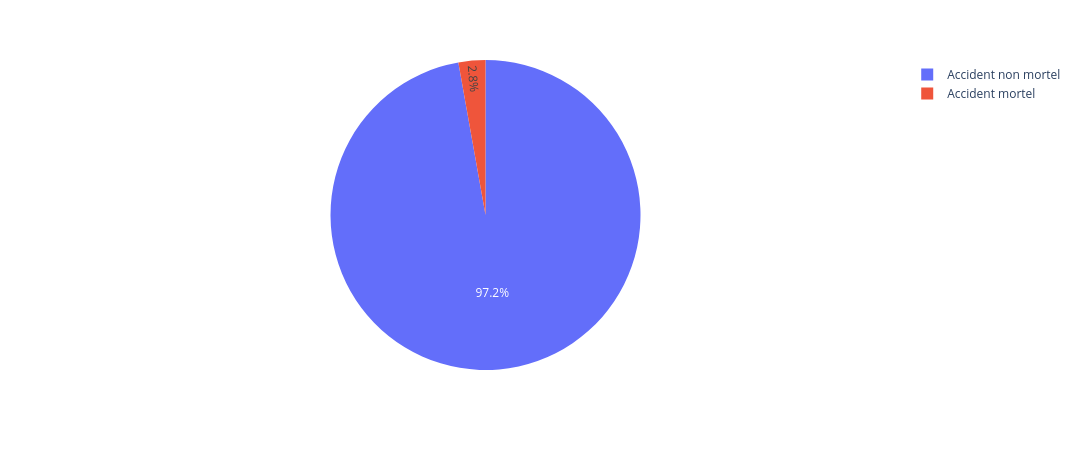
\includegraphics[width=12cm]{./img/grav1.png}
        \caption{Proportion d'accidents mortels}
    \end{figure}

    \section{Préparation des données}
    À partir des observations précédentes, nous avons supprimé les attributs moins intéressants pour l'apprentissage 
    et nous avons modifié certains attributs afin d'en extraire les informations intéressantes.
    \\
    Les attributs supprimés sont : \textit{voie}, \textit{v1}, \textit{v2}, \textit{pr}, \textit{pr1}, \textit{lartpc},
    \textit{larrout}, \textit{num\_veh}, \textit{occutc}, \textit{adr}, \textit{senc}, \textit{etatp}, \textit{actp}, 
    \textit{manv}, \textit{jour}, \textit{com}, \textit{hrmn}, \textit{motor}, \textit{place}, \textit{vosp}, \textit{locp}.
    \\\\
    Nous avons effectué les modifications suivantes :
    \begin{itemize}
        \item Création d'un attribut \textit{mortal} qui vaut 1 si le véhicule est impliqué dans un accident mortel, 0 sinon.
        \item À partir de l'attribut \textit{sexe}, nous avons créé un attribut \textit{sexe\_conducteur} qui garde seulement 
                le sexe du conducteur du véhicule.
        \item Création d'un attribut \textit{piéton} qui vaut 1 si un piéton est impliqué dans l'accident, sinon 0.
        \item Nous avons utilisé l'année de naissance et l'année de l'accident pour récupérer l'âge du conducteur.
        \item L'attribut \textit{vma} a été découpé en 4 catégories de vitesse.
        \item Pour les attributs \textit{catv} et \textit{catr}, nous avons gardé les valeurs les plus représentées dans la base de données.
    \end{itemize}
    \vspace{0.5cm}
    Nous avons également réduit les valeurs de certains attributs. Par exemple, pour des attributs 
    avec des valeurs telles que \textit{Non-renseigné}, \textit{Autre}, \dots \, nous avons regroupé 
    ces valeurs en une seule valeur. L'objectif était ici de simplifier en réduisant les catégories 
    mais également d'améliorer les performances de notre modèle.

    \section{Analyse des données}
    Une fois nos données préparées, nous avons pu les visualiser. Nous allons montrer dans les 
    deux prochaines parties les observations intéressantes que nous avons pu faire lors de 
    l'analyse de notre dataset.
    
    \subsection{Analyse univariée des données}
    \subsubsection{Les accidents mortels}
    Une donnée intéressante à observer est la proportion de véhicules impliqués dans un accident 
    mortel. C'est en effet la valeur que nous voulons prédire.

    \begin{figure}[ht]
        \centering
        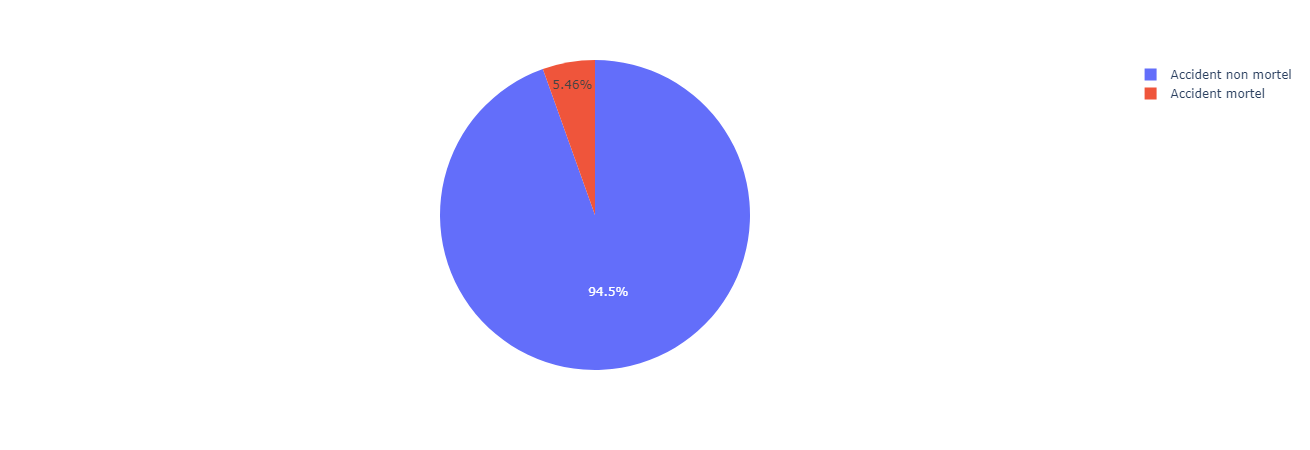
\includegraphics[width=10cm]{./img/grav2.png}
        \caption{Proportion des véhicules impliqués dans un accident mortel}\label{fig:fig_acc_mortel}
    \end{figure}

    Nous pouvons remarquer sur la figure \ref{fig:fig_acc_mortel} que le fait de s'intéresser 
    aux véhicules impliqués dans un accident mortel et non plus aux personnes nous permet 
    de doubler ce pourcentage. Même si cette proportion reste faible, cela va nous permettre 
    d'avoir plus de données dans la catégorie mortelle lors de l'apprentissage et par conséquent 
    d'avoir un meilleur modèle.

    \subsubsection{Les piétons}
    Nous nous sommes ensuite intéressés aux accidents dans lesquels un piéton est impliqué. 
    La figure \ref{fig:fig_acc_pieton} nous montre qu'un peu moins de 10\% des accidents impliquent 
    un piéton.

    \begin{figure}[ht]
        \centering
        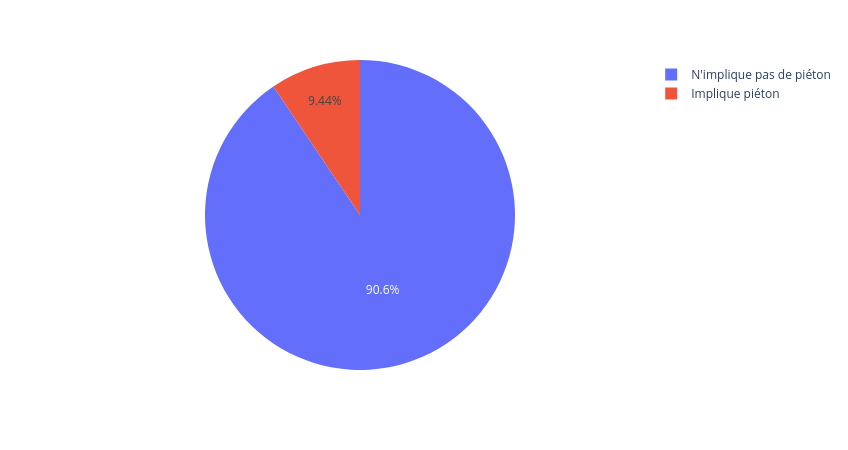
\includegraphics[width=10cm]{./img/pieton.png}
        \caption{Proportion des accidents avec piéton}\label{fig:fig_acc_pieton}
    \end{figure}

    \subsubsection{L'âge}
    Nous pouvons visualiser l'âge des conducteurs via une boîte à moustache. La figure \ref{fig:fig_age} nous 
    montre la répartition de l'âge des conducteurs. Lors du prétraitement des données, les valeurs aberrantes 
    ont été enlevées. On retrouve donc logiquement des âges contenus entre 0 et 100 ans. L'âge médian des 
    conducteurs est 33 ans avec le premier quartile à 21 et le troisième quartile à 49 ans. Même si on peut 
    imaginer que des valeurs sont fausses (il y a des conducteurs de moins de 16 ans), les valeurs sont tout de 
    même assez cohérentes par rapport à ce que l'on pourrait imaginer de la répartition de l'âge des conducteurs.

    \begin{figure}[ht]
        \centering
        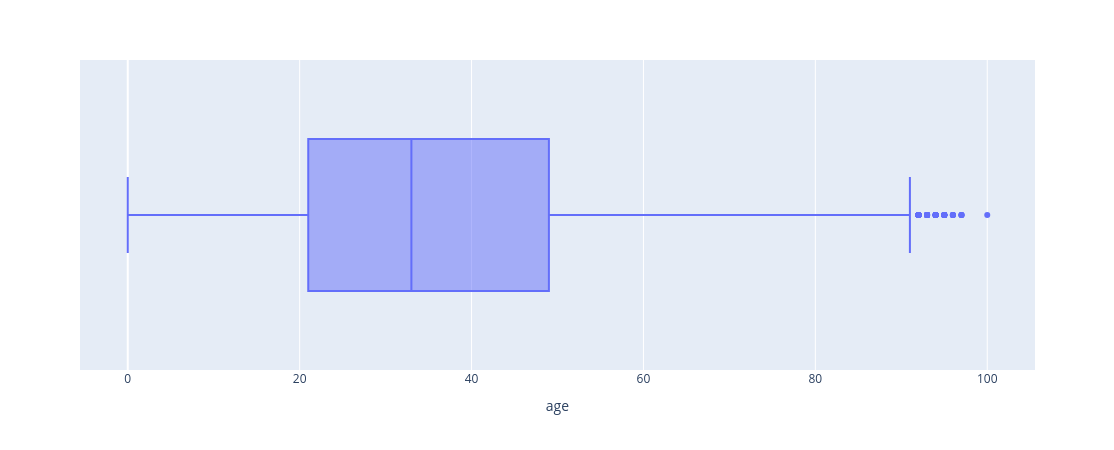
\includegraphics[width=12cm]{./img/age.png}
        \caption{Âge des conducteurs}\label{fig:fig_age}
    \end{figure}

    \subsubsection{Le genre des conducteurs}
    Le genre des conducteurs est assez intéressant à analyser. Sur la figure \ref{fig:fig_genre}, nous pouvons 
    remarquer une différence importante entre le nombre de femmes au volant d'un véhicule ayant eu un accident 
    (indice 0) et le nombre d'hommes (indice 1). Cette différence pourrait être une source de biais pour notre modèle. 
    En effet, le fait qu'il y ait beaucoup plus de données d'accident avec des hommes ne signifie pas qu'il y a plus 
    de chances d'avoir un accident si on est un homme. Cela signifie peut-être que la proportion d'hommes au volant 
    est plus élevée et donc qu'il y a plus d'accidents avec un homme au volant car il y a plus d'hommes au volant. Le 
    risque ici est que moins de données avec des femmes conduisent à des prédictions plus marquées pour les femmes et 
    par conséquent à des potentiels biais.

    \begin{figure}[ht]
        \centering
        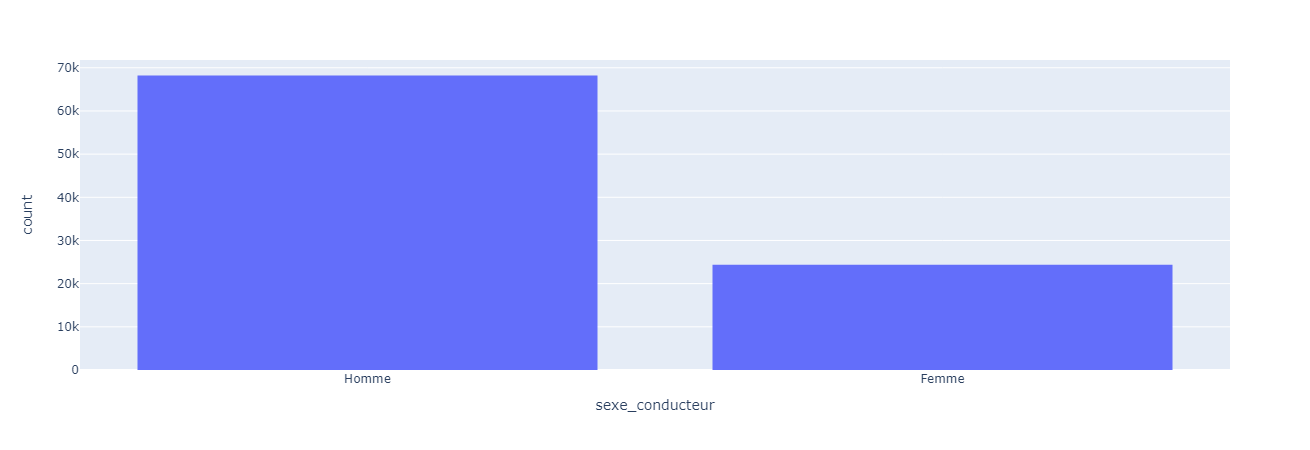
\includegraphics[width=12cm]{./img/sexe.png}
        \caption{Genre des conducteurs}\label{fig:fig_genre}
    \end{figure}

    \subsubsection{Le type de collision}
    La figure \ref{fig:fig_col} montre la répartition des différents types de collisions dans notre dataset. On peut 
    remarquer que tous les types de collisions sont plutôt bien représentés dans notre dataset. C'est un attribut qui 
    pourra être assez intéressant pour l'apprentissage.

    \begin{figure}[ht]
        \centering
        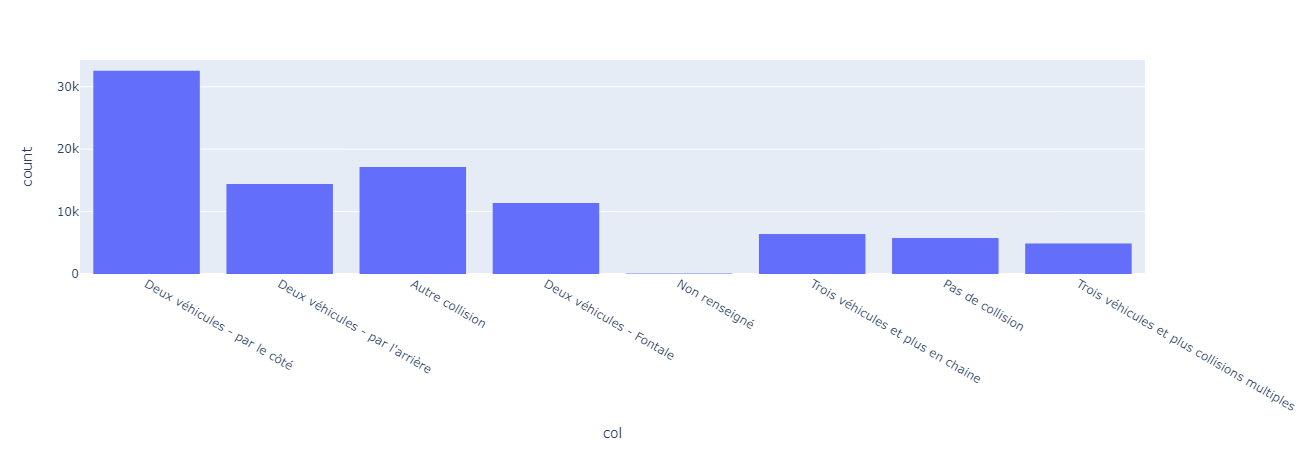
\includegraphics[width=12cm]{./img/col.png}
        \caption{Les types de collision}\label{fig:fig_col}
    \end{figure}

    \subsection{Analyse bivariée des données}
    Nous allons dans cette partie donner quelques exemples intéressants obtenus lors de l'analyse bivariée. On 
    peut retrouver l'ensemble des graphiques observés dans le fichier \texttt{main.ipynb}.

    \subsubsection{Le genre du conducteur}
    Un attribut qu'il est intéressant d'analyser est le genre du conducteur. En effet, il peut être source de biais 
    s'il y a un déséquilibre entre hommes et femmes.
    On retrouve globalement la même proportion dans la corrélation que l'on soit homme ou femme. Les hommes étant 
    beaucoup plus représentés dans le dataset, la proportion d'hommes est logiquement plus élevée. On peut cependant 
    faire quelques remarques. 
    
    La figure \ref{fig:fig_sexe_bivar1} nous montre une proportion de femmes moins élevée quand \textit{obsm} vaut 
    \textit{6}. La proportion de femmes est deux fois plus élevée quand \textit{obsm} vaut \textit{1}. Ceci pourrait biaiser notre 
    modèle.
    
    Sur la figure \ref{fig:fig_sexe_bivar2}, on remarque également une proportion différente de femmes 
    en fonction du type de véhicule. On pourrait expliquer cela par le fait que certains véhicules sont 
    dans la réalité plus utilisés par les hommes, par exemple on pourrait imaginer qu'il y a plus d'hommes qui 
    conduisent des motos. Il faudra être vigilant car cela peut être source de biais. Il se peut que notre 
    modèle associe une moto à un homme. Dans le cas d'une femme sur une moto le résultat pourrait être soit
    forcément un accident mortel, ou bien forcément un accident non mortel.

    \begin{figure}[h]
        \centering
        \begin{subfigure}{7cm}
            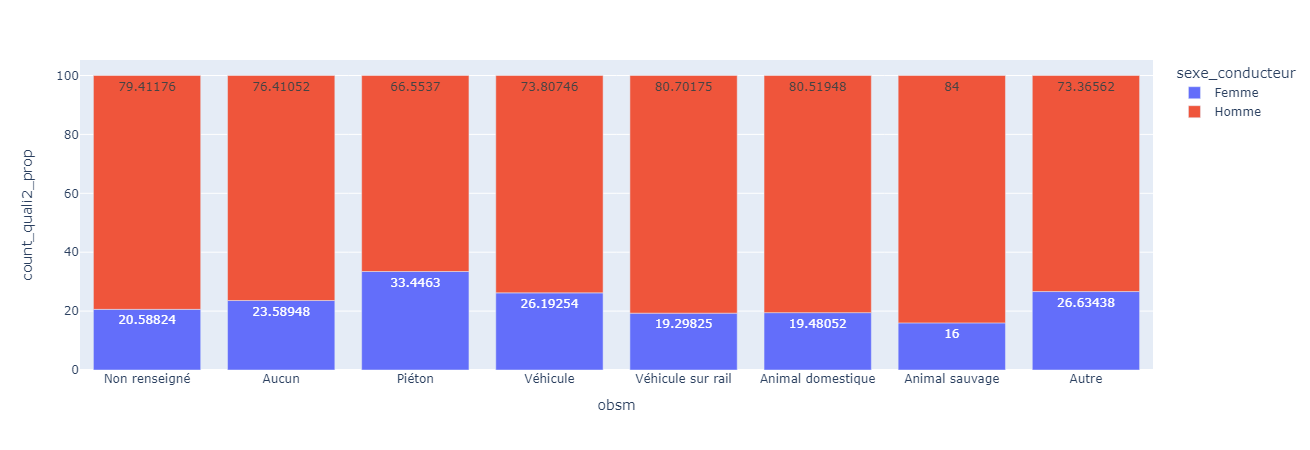
\includegraphics[width=7cm]{./img/bivar_sexe.png}
            \caption{Proportion femmes/hommes en fonction de la présence d'un obstacle dans l'accident}\label{fig:fig_sexe_bivar1}
        \end{subfigure}
        \hspace{0.2cm}
        \begin{subfigure}{7cm}
            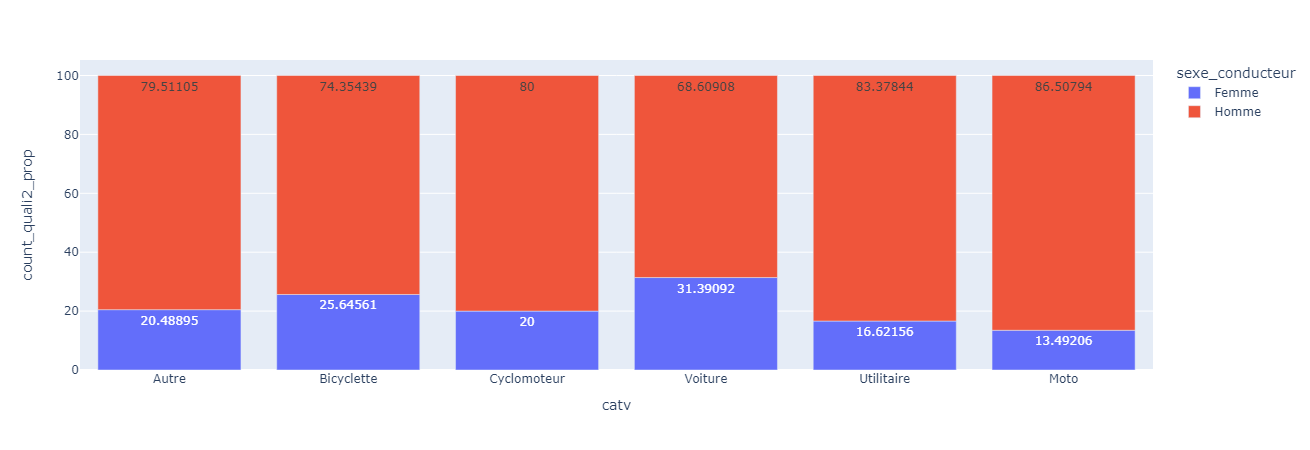
\includegraphics[width=7cm]{./img/bivar_sexe2.png}
        \caption{Proportion femmes/hommes en fonction de la catégorie du véhicule}\label{fig:fig_sexe_bivar2}
        \end{subfigure}
    \end{figure}
    \vspace{2cm}

    \subsubsection{L'âge du conducteur}
    On peut remarquer sur la figure \ref{fig:fig_age_bivar} que la probabilité d'accident mortel est beaucoup plus élevée à l'âge de 
    21 ans. Cela est dû en partie au fait que les conducteurs de 21 ans sont surreprésentés. Cette probabilité risque de poser 
    problème pour notre modèle. En effet l'âge n'est pas un paramètre déterminant dans l'évaluation de la gravité de l'accident. 
    Le problème est que notre modèle va probablement associer l'âge de 21 ans à un accident mortel, peu importe les autres paramètres 
    de l'accident. L'âge serait donc notre \textbf{attribut sensible}.

    \begin{figure}[ht]
        \centering
        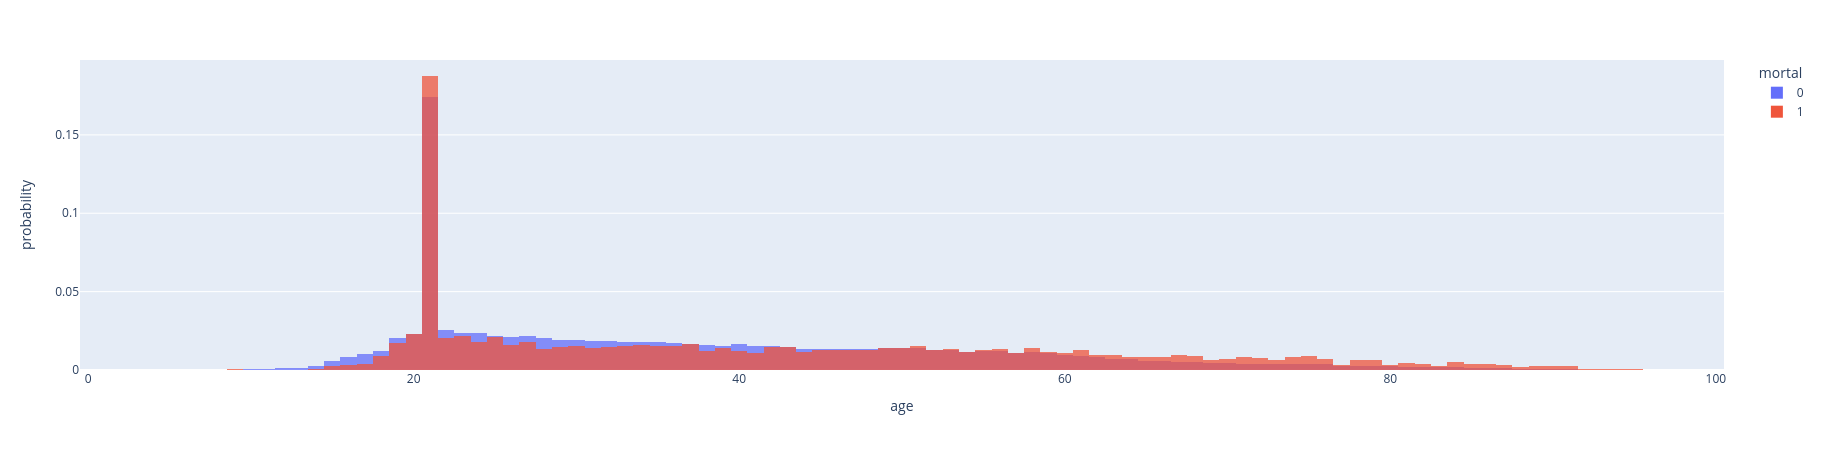
\includegraphics[width=14cm]{./img/bivar_age.png}
        \caption{Analyse bivariée âge -- accident mortel}\label{fig:fig_age_bivar}
    \end{figure}
    
    \section{Apprentissage}
    
    \subsection{Split}
    Séparer nos données en deux ensembles demandait de tenir compte d'une spécificité. Nous nous plaçons du point de vue d'un véhicule, 
    mais bien souvent, plusieurs véhicules sont impliqués dans un  même accident. Il nous a donc fallu adapter le split pour que les 
    véhicules d'un même accident soient dans le même ensemble. 
    
    Par ailleurs, nous avons constaté que, si on ne le faisait pas, un surapprentissage lors du test se produisait. Typiquement, un trop grand 
    nombre de morts étaient correctement prédits. Mais le modèle trouvait une partie de ces véhicules en les associant à ceux avec lesquels
    ils avaient eu un accident dans l'ensemble d'apprentissage. 
    
    \subsection{Encodage One Hot}
    La base de données nous fournit, pour la plupart des attributs, des données qui peuvent être converties en entiers. 
    Par exemple, une catégorie de véhicule (\textit{catv}) est désignée par un chiffre. L'attribut reste cependant catégoriel. En pratique, 
    les seuls attributs quantitatifs qui nous restent sont l'âge du conducteur, les mois et les départements. 
    Le reste est soit binaire, soit qualitatif. 
    
    Tous les attributs qualitatifs ont donc été transformés en OneHot. Initialement, nous souhaitions optimiser le nombre de colonnes en 
    réalisant les OneHot nous-mêmes. Par exemple, prenons "surf" (l'état de la surface de la route). Il est inutile de créer une colonne 
    pour "Non-renseigné", "Autre" ou "normale". Nous sommes uniquement intéressés par les états spécifiques de la route. 
    
    Cependant, cette approche posait des problèmes car elle empêchait la réalisation de l'audit. Nous avons donc utilisé la méthode 
    standard pour nos OneHot. 
    
    \subsection{Arbre de décision}
    Une fois les données prêtes, nous avons utilisé le classifieur par arbres de décision pour obtenir un modèle. C'est le premier que nous 
    avons utilisé. En ce qui concerne les résultats, le score d'accuracy est de \textit{1} pour l'entraînement et de \textit{0.9014} pour le test.
        
    En ce qui concerne la matrice de confusion, on remarque que \textit{27687} véhicules ont été classés correctement en tant qu'accidents non létaux.
    Tandis que \textit{291} accidents mortels seulement ont été correctement identifiés. Cependant, \textit{1413} accidents mortels ont été recensés à tort 
    comme étant non létaux et \textit{1648} véhicules ont subi le sort inverse. 
    
    \begin{figure}[h]
        \centering
        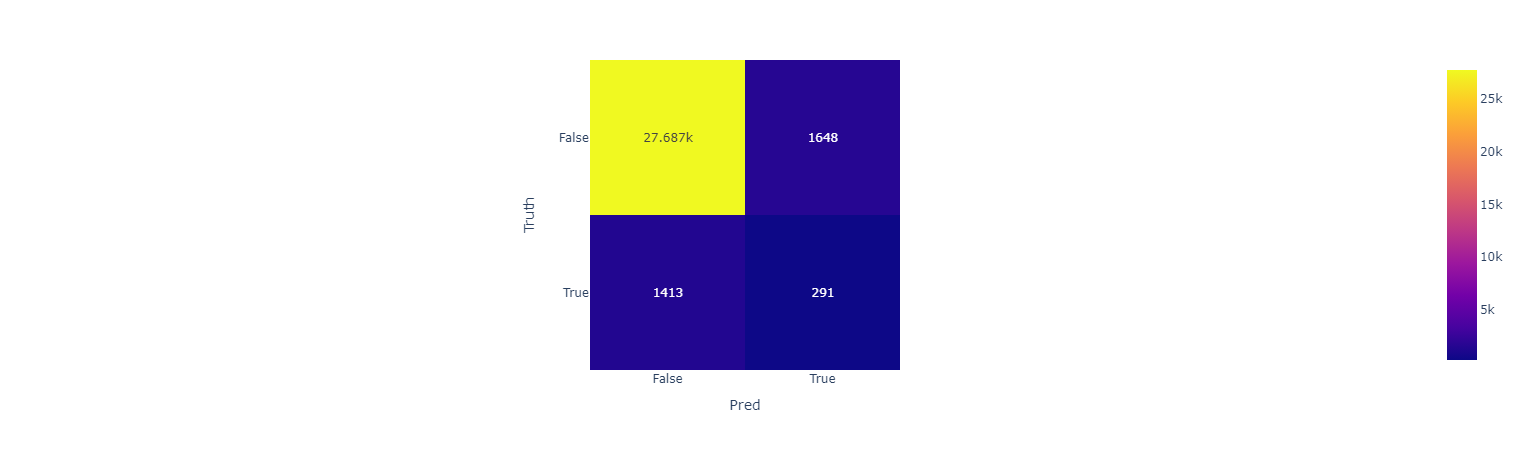
\includegraphics[width=\textwidth]{./img/matrice_confusion_tree.png}
        \caption{La matrice de confusion pour le classifieur d'arbres aléatoires}
    \end{figure}
    

    En résumé, on remarque que le modèle réussit très bien à classifier les accidents qui n'ont pas conduit à la mort de quelqu'un. Cependant, 
    il lui apparaît bien plus difficile de trouver les véhicules impliqués dans des accidents mortels. On peut attribuer ceci au fait que ces 
    accidents létaux ne représentent que \textit{5.38\%} des véhicules accidentés répertoriés dans la base.

    \subsection{GaussianNB}
    Avancés dans le projet, nous avons voulu tester plusieurs classifieurs, tous ont donnés des résultats différents, pour certains médiocres. 
    Mais nous avons trouvé un autre classifieur qui donnait des résultats intéressants : GaussianNB.
        
    Il ne maximise pas notre accuracy score puisqu'il n'est que de \textit{0.8734} à l'entraînement et de \textit{0.8677} pour les tests. Ce qui 
    a toutefois retenu notre attention, c'est le nombre d'accidents létaux qu'il parvient à détecter : \textit{508}. Réduisant ainsi l'erreur associée
    (les accidents mortels recensés à tort comme étant non létaux) à seulement \textit{1196}. Ceci s'accompagne malheureusement une perte de performances 
    pour ce qui est de la détection d'accidents non mortels comme on peut le voir ci-dessous.

    \begin{figure}[h]
        \centering
        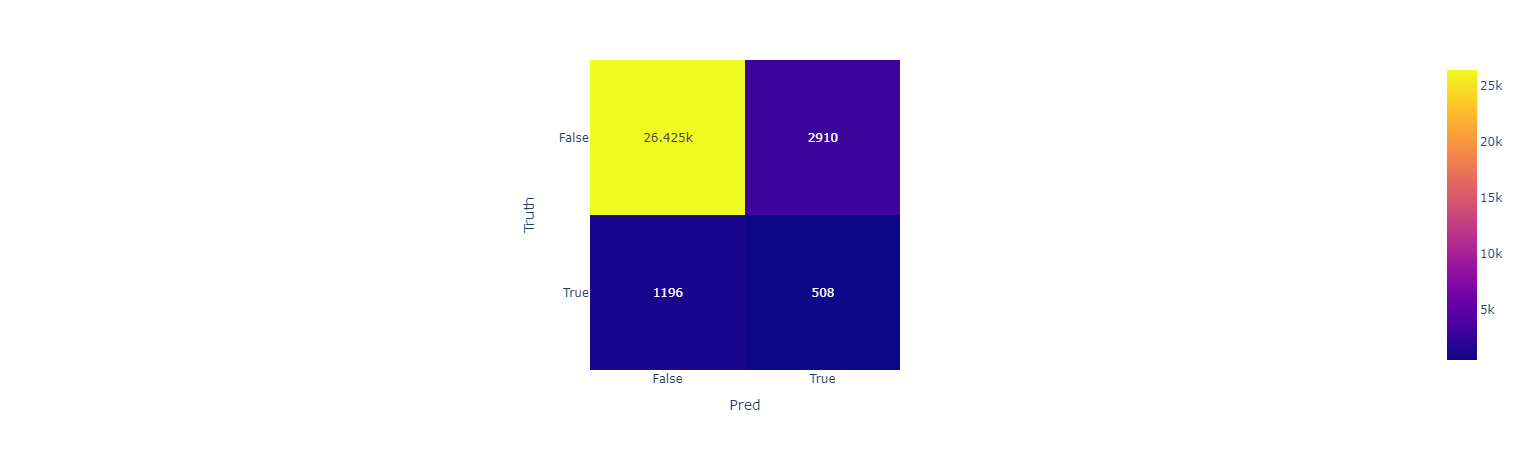
\includegraphics[width=\textwidth]{./img/matrice_confusion_gaussien.png}
        \caption{La matrice de confusion avec GaussianNB}
    \end{figure}

    Un autre avantage qui peut ressembler à un inconvénient au départ est que ce classifieur demande des nombres et non des OneHot.
    Nos valeurs au départ sont en format numérique, rendant donc nos données compatibles avec cette approche.
    Ceci nous ouvre alors la possibilité de tester d'autres choses puisque le classifieur donne des probabilités et non des arbres. Au premier 
    rang desquels \textit{xplique}.
        
    Par souci de concision cependant, nous prendrons le modèle issu du \textit{tree classifier} pour tous les audits qui vont suivre, 
    puisque c'est le premier avec lequel nous avons travaillé. On notera tout de même que lorsqu'on effectue ces audits avec \textit{GaussianNB}, 
    les résultats diffèrent en bien des points de ceux observés avec le \textit{tree classifier}, preuve qu'ils ont une approche bien différente.

    \subsection{Base Rate}

    Nous avons voulu mesurer les résultats méritant potentiellement une protection : le fait qu'un piéton soit impliqué dans 
    un accident et le sexe du conducteur. Voici les résultats :

    \begin{itemize}
        \item \textbf{Sexe du conducteur} 1 (un homme)
        \item \textbf{Disparate Impact} : 1.21767750298587 1.6331199049428085
        \item \textbf{P-rule disparate Impact} : 0.8212355057458954 0.6123249107266375
        \item \textbf{Démographie Parité} : 0.011747835864606336 0.02383701239031672
    \end{itemize}

    Ce qui est flagrant ici, c'est qu'il existe une disparité dans la prédiction d'accidents mortels pour les hommes. Allant par ailleurs
    dans le sens de ce qu'indique Disparate Impact par la suite. Notons cependant que la disparité démographique entre hommes et femmes
    existe mais est très faible.

    \begin{itemize}
        \item \textbf{Piéton} 1 (un piéton est impliqué)
        \item \textbf{Disparate Impact} : 1.0538191011165416 1.0968113720110815
        \item \textbf{P-rule Disparate Impact} : 0.9489294689576994 0.9117337999207913
        \item \textbf{Démographie Parité} : 0.003345154811069756 0.005266913173450724
    \end{itemize}

    Pour ce qui est de l'implication d'un piéton dans un accident, on constate ici aussi une légère disparité, soulignant leur
    plus grande implication dans des accidents mortels. Ceci concorde encore une fois avec le \textit{disparate Impact}. Démographiquement, 
    le cas est similaire au sexe, puisqu'on constate une légère disparité en leur faveur, bien que cette fois la disparité soit plus
    faible encore.

    \section{Audit du modèle}

    \subsection{Génération des contrefactuels avec Dice}
    Dice nous a permis d'établir quels attributs influent sur la prédiction de notre modèle. Les résultats sont 
    cependant assez variables d'une exécution à l'autre. On peut tout de même retrouver lesquels sont fréquemment impliqués 
    dans le changement des exemples contrefactuels.
    Parmi eux, on peut noter que l'attribut \textit{âge} est souvent représenté. Le taux d'accidents (notamment mortels) étant plus 
    élevé chez les jeunes et les personnes âgées, cela paraît assez cohérent. L'attribut \textit{obsm} est également 
    souvent utilisé dans les exemples contrefactuels.
    Nous avons pu remarquer que l'attribut \textit{col} est peu représenté dans les résultats, contrairement à l'hypothèse que 
    nous avions pu faire lors de l'analyse.

    Enfin, les attributs \textit{dep} et \textit{sexe\_conducteur} sont également représentés. Ils pourraient être sources de biais, notamment 
    l'attribut \textit{dep} ; le modèle pourrait associer un département à une prédiction d'accident mortel.


    \subsection{BlackBoxAuditing}
    Les résultats que nous allons analyser sont issus du modèle généré par \textit{tree classifier}.

    Tout d'abord, l'audit a porté sur les 24 features que nous avons conservé afin d'élaborer ce modèle. 
    On constate tout d'abord le rôle prédominant de l'âge pour l'accuracy score. À \textit{0.84}, ce dernier éclipse 
    tous les autres. Une explication pourrait venir de ce que nous avons constaté dans notre analyse univariée : il y a une 
    surreprésentation des jeunes de 20--21 ans dans ce set. Ceci est en réalité loin de surprendre puisqu'il s'aligne avec la 
    politique de prix pratiquée par les assureurs envers les jeunes conducteurs.

    Par la suite, on peut s'intéresser à l'évolution de l'accuracy en fonction du niveau de réparation appliqué à chaque 
    attribut :

    \begin{figure}[h]
        \centering
        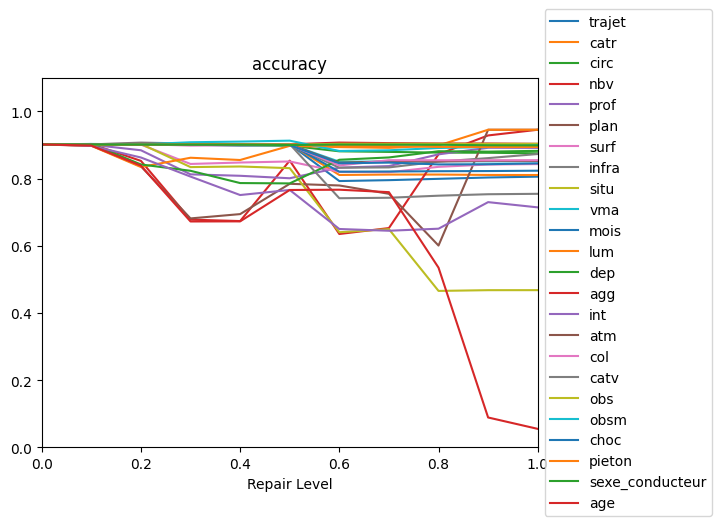
\includegraphics[width=10cm]{./img/accuracy.png}
        \caption{L'accuracy en fonction du niveau de réparation pour chaque attribut.}
    \end{figure}

    On reconnaît toput de suite les 
    attributs dont l'accuracy est au plus haut en regardant ceux qui s'effondrent le plus. En premier lieu, l'âge s'illustre
    à nouveau. À la lumière de ceci, il apparaît évident que le modèle discrimine fortement les véhicules en fonction de l'âge du 
    conducteur. Dans une moindre mesure, on constate la même chose pour \textit{situ}, qui fait référence à la localisation 
    géographique de l'accident. Ce qui paraît sensé, étant donné que certains lieux sont plus dangereux que d'autres. Enfin, 
    on observe que le type d'intersection et la catégorie du véhicule sont également sources de discriminations de la part de notre 
    modèle. Encore une fois, cela semble cohérent.

    Toutefois, notons l'absence de quelques attributs notables tels que le nombre de voies, le sexe du conducteur (chose intéressante :
    ce n'est pas le cas avec GaussianNB), le type de collision, le type d'obstacle heurté ou encore le fait qu'un piéton soit impliqué.
    
    Maintenant regardons l'équilibre du modèle à l'aide du BCR.

    \begin{figure}[h]
        \centering
        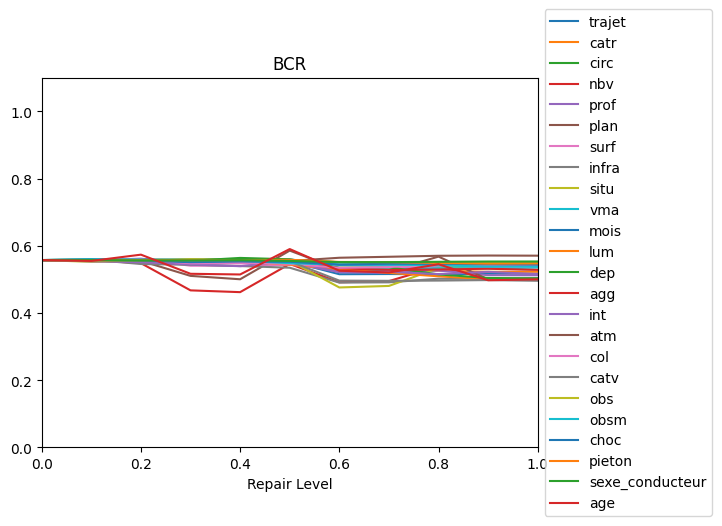
\includegraphics[width=10cm]{./img/BCR.png}
        \caption{Le BCR en fonction du niveau de réparation pour chaque attribut.}
    \end{figure}

    On remarque ici que les attributs sont plutôt centrés autour de \textit{0.5} et que la plupart reste rectiligne, mais que certains divergent
    quelque peu. Cet évasement est dû à des attributs déjà connus tels que \textit{âge} ou \textit{catv}. D'autres influent aussi mais ne s'étaient pas 
    illustrés précédemment, à l'image du nombre de voies (\textit{nbv}), du profil de la route (\textit{plan}) ainsi que de la luminosité (\textit{lum}). 

    Malgré cela, l'évasement assez faible laisse penser que le modèle est plutôt équilibré. De plus, comme mentionné précédemment 
    dans la section dédiée au split, nous avons pu tester le cas où l'on acceptait que des véhicules impliqués dans le même accident
    se retrouvent dans des ensembles différents (entraînement / test). Ce qu'il ressortait alors du BCR était un évasement beaucoup
    plus important et une origine située vers 0.68. Ce qui laisse à penser que cette version était bel et bien trop modelée sur le train
    set, l'équilibre était rompu.

    Pour conclure, BlackBoxAuditing nous a permis de comprendre quels étaient les attributs les plus discriminés. Âge est certainement le plus notable.

    \subsection{Expliquer le modèle avec les valeurs de Shapley}
    Afin d'analyser la contribution des différents attributs dans notre modèle, nous avons 
    utilisé les valeurs de Shapley. Nous avons d'abord essayé de calculer la valeur exacte avec la fonction 
    \verb|ShapleyValues| du module \textit{ShapKit}. Cependant, le nombre d'attributs de notre dataset est trop 
    important et le calcul trop long.
    Il a donc fallu calculer une approximation de la valeur de Shapley avec la fonction \verb|MonteCarloShapley|.
    Nous devons cependant être prudents car ce calcul de l'approximation nous 
    donne une tendance pour notre modèle mais certainement pas une valeur exacte. On peut le constater en changeant 
    le nombre d'itérations, qui produit souvent un résultat différent. Toutes les approximations ont ici été calculées 
    avec \texttt{n\_iter=1000}.

    Le temps de calcul étant encore assez long nous avons parallélisé le calcul des valeurs de Shapley. Les calculs 
    ont ensuite été séparés en deux, d'un côté pour les prédictions qui donnent 1 et de l'autre pour celles qui donnent 0.
    ON peut ainsi avoir une idée des attributs décisifs dans les deux cas.

    Ce qui ressort des résultats obtenus est que les attributs \textit{col}, \textit{choc}, \textit{obsm}, \textit{int} 
    et \textit{agg} contribuent souvent au résultat. Ce résultat paraît plutôt cohérent.
    En revanche, on retrouve également assez souvent les attributs \textit{mois}, \textit{âge} et \textit{dep}. Ces 
    attributs ne devraient pas contribuer autant à la sortie de notre modèle. Il peuvent constituer un biais (ce n'est 
    pas parce qu'on a un accident à l'âge de 21 ans que l'on va forcément mourir, d'autres attributs sont beaucoup plus 
    importants).


    Pour l'attribut \textit{sexe\_conducteur} on nous donne une contribution 
    nulle de cet attribut. Cela peut nous encourager dans l'idée que le sexe n'est pas un biais pour notre modèle 
    conrairement à ce que nous pouvions penser au départ.

    Ci-dessous un résultat obtenu du calcul des valeurs de Shapley. Vous pouvons retrouver un échantillon des résultats dans l'annexe ? de ce rapport.
    
    

    \begin{figure}[h]
        \centering
        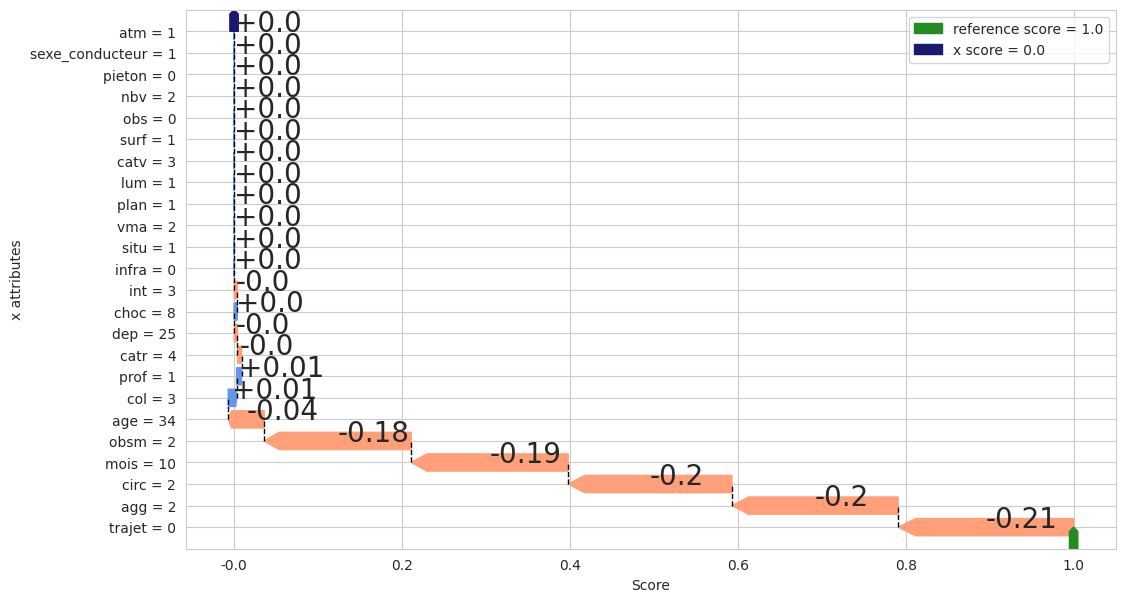
\includegraphics[width=\textwidth]{./img/shap1.png}
        \caption{Une approximation des valeurs de Shapley}
        \label{fig:fig_shap}
    \end{figure}

    \subsection{Expliquer le modèle avec Lime}
    Nous avons également utilisé \textit{Lime} afin d'avoir une idée des attributs qui contribuent
    le plus aux prédictions de notre modèle. On peut retrouver le code correspondant dans le fichier 
    \texttt{lime.ipynb}.

    Nous avons d'abord récupéré les indices des prédictions positives de notre modèle (avec lesquelles les 
    entrées notre modèle prédit 1). Ainsi, on a pu regarder dans les cas où les prédictions sont 0 
    et les cas où les prédictions sont 1.
    On peut remarquer qu'on trouve des variables similaires à celles trouvées avec les valeurs de 
    Shapley. On retrouve notamment assez fréquemment l'attribut \textit{agg}.
    Cependant, contrairement au résultat que pouvait nous donner \textit{ShapKit}, l'attribut \textit{mois} est 
    moins représenté. Les contributions sont également plus réparties entre les attributs.
    Enfin, il semble que, comme nous avions pu l'observer avec les valeurs de Shapley, l'attribut 
    \textit{sexe\_conducteur} ait un faible impact sur la prédiction.

    \section{Premières conclusions}
    Pour ce projet nous avons cherché un dataset qui nous intéressait, et nous avons choisi celui rapportant les accidents de la route. Pourvu de 
    nombreux attributs, nous avons dû adapter leur format avant de pouvoir les analyser de manière univariée puis bivariée. Lors du premier essai, 
    nous avons fait le choix d'utiliser des arbres de décision. Ce qui nous a conduit à transformer beaucoup de nos variables en OneHot. L'accuracy 
    de ce modèle était élevée, mais il a du mal à trouver les accidents réellement mortels. Pour ce modèle, nous avons par la suite calculé le base 
    rate puis effectué quelques audites tels que dice, BlackBoxAuditing et shapkit.

    Par la suite nous avons essayé de trouver un classifieur qui avait de meilleures performances, c'est ainsi que nous avons trouvé GaussianNB, qui
    est meilleur pour détecter les véhicules impliqués dans des accidents vraiment mortels. Pour ce modèle nous avons aussi effectué les audits 
    évoqués précédemment, mais nous ne les avons pas analysés dans ce rapport. Ce qui conclut notre premier rendu. 

    L'analyse des données puis les audits que nous avons effextués après entrainement du modèle nous ont permis d'identifier 
    plusieurs attributs sensibles. D'abord nous pensions que le genre du conducteur pourrait avoir un impact sur la prédiction. 
    Cela aurait été un biais de notre modèle. Or nous avons pu observer via les différents outils utilisés que le genre du 
    conducteur a un impact très faible sur la prédiction du modèle. En revanche, le travail effectué nous a permis d'identifier 
    d'autres attributs sensibles qui eux ont réel impact sur les sorties du modèle. Les attributs \textit{âge}, \textit{dep} et 
    \textit{mois} sont des attributs que nous avons identifié comme sensibles pour notre modèle. Ils ont un impact assez important 
    sur les prédictions et pourtant ne devraient pas être décisifs dans la classification d'un accident mortel ou non mortel.

    \section{Une réflexion pour la suite}
    Cette première partie nous a permis de nous familiariser avec notre jeu de données. L'objectif de classification a été une 
    question qui nous a suivi du début de ce projet jusqu'à la rédaction de ce rapport. 
    Les premières conclusions nous ont mené encore une fois à la réflexion sur une nouvelle direction à suivre pour la classification. 
    Ne faudrait-il pas classifier l'ensemble des 
    gravité ? Nous nous basons dans cette première partie sur des données dans lesquelles nous avons seulement 5\% d'accidents 
    mortels. Ne serait-il pas judicieux de prendre en compte l'ensemble de gravité et donc de travailler sur des proportions 
    plus conséquentes ?

    Ces questions seront déterminantes pour la suite de ce projet.

    \newpage
    \part{Correction des biais}

    \section{Améliorations du modèle}
    Cette deuxième partie du projet a commencé par l'amélioration des premiers resultats. Nous allons parcourir 
    dans cette section les différentes amélioration effectuées avant d'arriver à la correction des biais.

    \subsection{Nouvelle métrique de base : taux d'erreur et de justesse}

    Afin de trouver l'attribut à protéger et pour mieux diagnostiquer les effets des différentes méthodes de réduction de
    biais, nous avons mis en place une nouvelle métrique de base. En tout il y a 4 calculs : 

    \begin{itemize}
        \item Taux d'\textbf{erreur} pour l'attribut \textbf{sensible} : \[ P(\overline{Y}=1| (Y=0, Z=1)) \]
        \item Taux d'\textbf{erreur} pour l'attribut \textbf{privilégié} : \[ P(\overline{Y}=1| (Y=0, Z=0)) \]
        \item Taux de \textbf{justesse} pour l'attribut \textbf{sensible} : \[ P(\overline{Y}=1| (Y=1, Z=1)) \]
        \item Taux de \textbf{justesse} pour l'attribut \textbf{privilégié} : \[ P(\overline{Y}=1| (Y=1, Z=0)) \]
    \end{itemize}

    Seules, ces métriques n'ont que peu d'intérêt, c'est lorsqu'on les regarde ensemble qu'elles prennent tout leur intérêt pour 
    la fairness. En effet, l'équité est garantie si la différence entre ces taux pour l'attribut sensible et l'attribut privilégié 
    est nulle. En effet on serait en droit de s'attendre à ce que la justesse et l'erreur se produisent dans les mêmes proportions. 
    Notons pour finir que la liste des taux de succès est incomplète. On aurait pu ajouter le cas $\overline{Y}=0| Y=0$, mais ce n'est pas ce qui 
    nous intéresse le plus dans notre cas. On souhaite se concentrer sur les prédictions d'accidents mortels.

    \subsection{Sur-échantillonnage}
    Le prétraitement des données a été amélioré avec l'utilisation de l'outil de sur-échantillonnage \textit{SMOTE}.
    Nous avions pu remarquer lors de l'analyse de nos données que les accidents mortels sont minoritaires (environ $5\%$).
    Cet outil nous permet de rééquilibrer les classes afin d'avoir un meilleur apprentissage sur la classe des accidents 
    mortels. \textit{SMOTE} va générer de nouveaux individus minoritaires qui ressemblent à ceux déjà présents sans 
    pour autant être identiques.
    Nous pouvons voir sur la figure~\ref{fig:smote1} que le rééquilibrage nous donne 50\% pour chaque classe 
    tout en affectant peu les proportions sur les autres attributs comme nous le montre la figure~\ref{fig:smote2} 
    qui prend pour exemple l'attribut \textit{sexe\_conducteur}.
    Les résultats observés sont bien plus concluants en utilisant cette méthode.
    Tous les résultats obtenus dans la suite utilisent donc cette méthode lors du prétraitement.
    \\\\
    \begin{figure}[!h]
        \vspace{2cm}
        \centering
        \begin{subfigure}{7cm}
            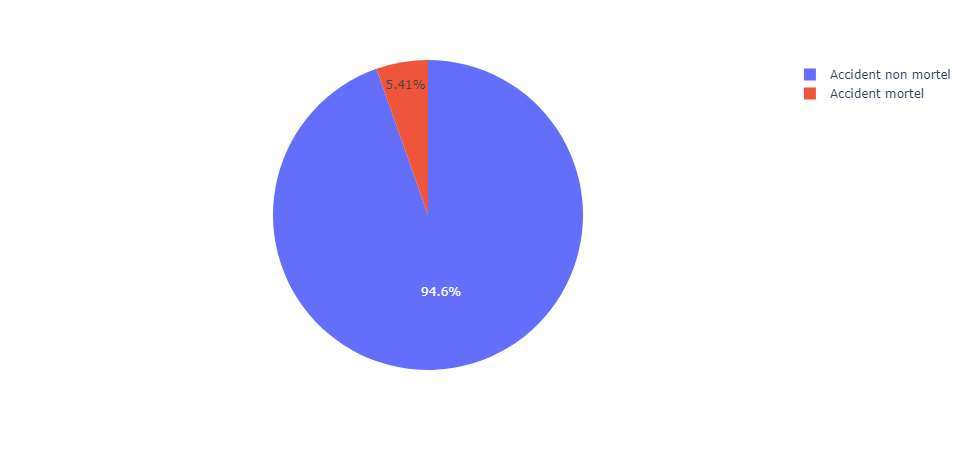
\includegraphics[width=7cm]{./img/smote/before.png}
            \caption{Accidents mortels avant SMOTE}\label{fig:before_smote}
        \end{subfigure}
        \hspace{0.2cm}
        \begin{subfigure}{7cm}
            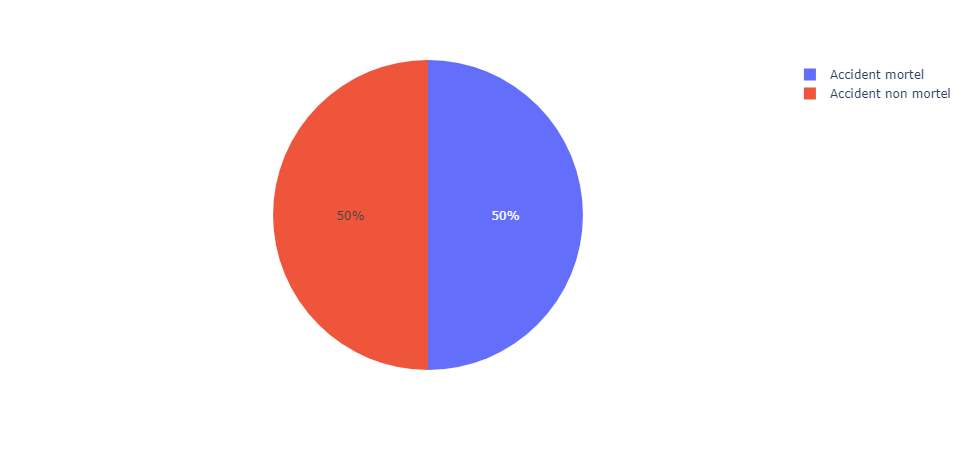
\includegraphics[width=7cm]{./img/smote/after.png}
        \caption{Accidents mortels après SMOTE}\label{fig:after_smote}
        \end{subfigure}
        \caption{Accidents mortels avant/après SMOTE}\label{fig:smote1}
    \end{figure}
    \vspace{1cm}
    \begin{figure}[h]
        \centering
        \begin{subfigure}{6cm}
            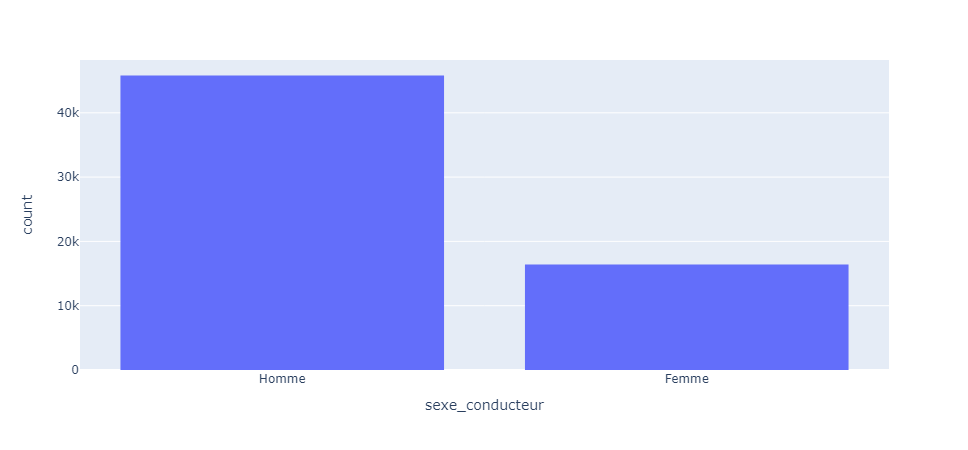
\includegraphics[width=6cm]{./img/smote/sex_before.png}
            \caption{Homme/Femme avant SMOTE}\label{fig:before_smote_sex}
        \end{subfigure}
        \vspace{\floatsep}
        \hspace{0.4cm}
        \begin{subfigure}{6cm}
            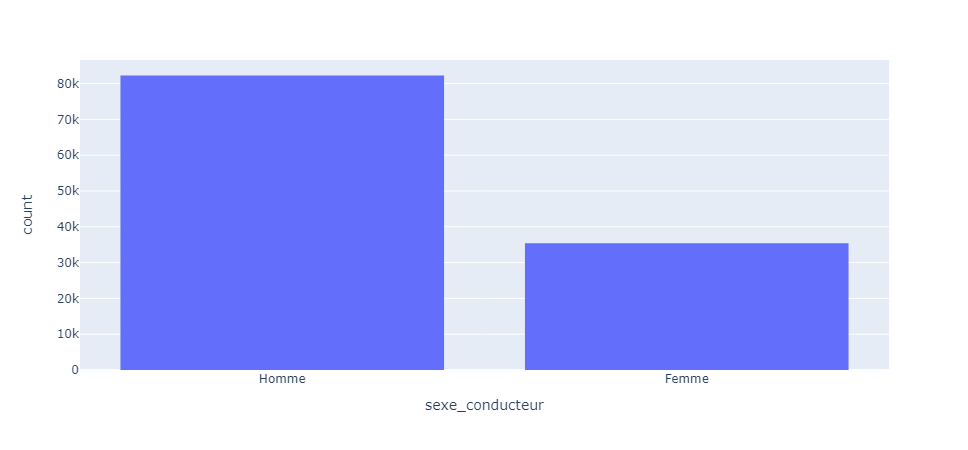
\includegraphics[width=6cm]{./img/smote/sex_after.png}
        \caption{Homme/Femme après SMOTE}\label{fig:after_smote_sex}
        \end{subfigure}
        \caption{Proportion Homme/Femme avant et après SMOTE}\label{fig:smote2}
    \end{figure}
    \vspace{1cm}

    \subsection{\textit{Random Forest Classifier}}
    La première partie de ce projet utilisait un \textit{Decision Tree Classifier}.
    Afin d'avoir un modèle plus robuste, nous avons décidé d'utiliser une forêt aléatoire.
    À première vue, les résultats étaient bien moins bons. En effet le nombre de 
    vrais positifs est très faible. Cependant, en modifiant le seuil d'acceptation on 
    peut faire évoluer la quantité de vrais positifs et obtenir des résultats bien plus 
    intéressants. Une classe a été créée afin de surcharger la méthode \verb|predict| de 
    la classe \textit{RandomForestClassifier}. Après plusieurs essais sur différentes valeurs, 
    le seuil a été fixé à $0.2$. 

    \subsection{Attributs sensibles}
    L'analyse du nouveau modèle nous a mené à de nouvelles observations. D'abord, nous avons 
    remarqué une réduction du disparate impact pour le sexe féminin. De plus, les différents 
    outils d'évaluation des biais nous montrent que le sexe féminin est plus discriminé sur 
    ce modèle. D'un autre côté, l'utilisation de ce modèle a eu pour effet de réduire l'influence de 
    l'âge, le mois et le département sur la prédiction, ce qui est un point positif. Nous pouvons notamment 
    l'observer au travers des valeurs de Shapley obtenues avec ce nouveau modèle. 
    
    Dans la suite de ce projet nous nous penchons 
    donc sur la correction des biais de l'attribut \textit{sexe\_conducteur}.



    \section[Preprocessing]{Pre-processing\footnote{Le pre-processing a été effectué sur un modèle avec seuil (0.2)}}
    \subsection{Repondération}
    Dans le contexte de la fairness, la repondération a pour objectif de rééquilibrer le set d'entrainement
    en attribuant des poids différents à chaque instance. Ce poids est calculé en fonction de l'impact 
    que cette instance a sur l'attribut sensible. 
    Après apprentissage et observation des résultats de notre modèle, nous pouvons faire deux 
    observations. Premièrement les métriques de fairness sont très positives. Le disparate impact 
    passe de $0.50$ à $0.94$ pour les femmes. La seconde observation est que l'accuracy de notre 
    modèle a en revanche diminuée de $0.87$ à $0.75$. Cela peut s'expliquer par une augmentation 
    du nombre de faux positifs. D'un autre côté, un point intéressant est que le nombre de 
    vrais positifs est maintenant plus élevé que le nombre de faux négatifs, ce qui n'était pas 
    le cas sur les modèles testés jusqu'ici.
    La matrice de confusion (figure~\ref{fig:reweight_matrix}) nous montre 
    les résultats obtenus après repondération. En
    résumé ce nouveau modèle catégorise trop d'accidents comme étant mortels. Mais parmi les accidents détectés comme
    étant mortels seul un sur huit l'est vraiment. Dans notre cas c'est intéressant car dans un objectif de prévention
    routière, on veut écarter les causes d'accidents non mortels des campagnes de sécurité pour augmenter leur efficacité.

    \begin{figure}[h]
        \centering
        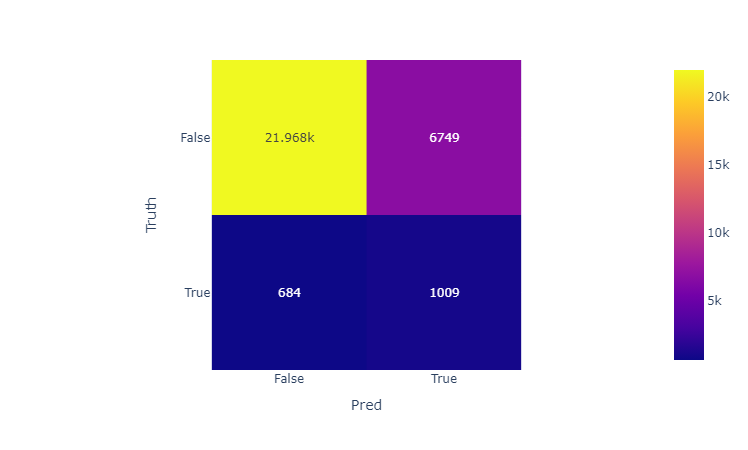
\includegraphics[scale=0.4]{./img/confusion_matrix_reweight.png}
        \caption{Matrice de confusion avec repondération}
        \label{fig:reweight_matrix}
    \end{figure}

    %\vspace{6cm}
    \subsection{Disparate Impact Remover}
    Les résultats obtenus avec le \textit{Disparate impact remover} sont similaires à ceux obtenus avec 
    la repondération. On obtient une accuracy de $0.75$ et un disparate impact de $0.89$. Le disparate 
    impact est cependant un peu moins bon que celui obtenu avec la repondération pour une accuracy équivalente.
    On peut remarquer que tout comme avec la repondération, la matrice de confusion (figure~\ref{fig:DIR_matrix})
    nous montre une tendance allant vers plus de faux positifs. On remarque également encore une amélioration
    des prédictions de vrais positifs qui est très proche de celle obtenue par la méthode précédente.
    Le disparate impact remover peut être réglé avec un paramètre \textit{level}. La figure~\ref{fig:DIR_param} 
    nous montre que le disparate impact reste plutôt stable sauf avec les paramètres $0.6$ et $0.7$.
    La valeur la plus élevée est de $0.89$ avec $level=0.9$. Les résultats obtenus avec ce modèle étant très proches 
    de ceux avec la repondération, on préférera utiliser la repondération dont l'entrainement est plus rapide l'adaptation 
    à notre modèle plus simple.
    %\vspace{4cm}

    \begin{figure}[!h]
        %\vspace{2cm}
        \centering
        \begin{subfigure}{8cm}
            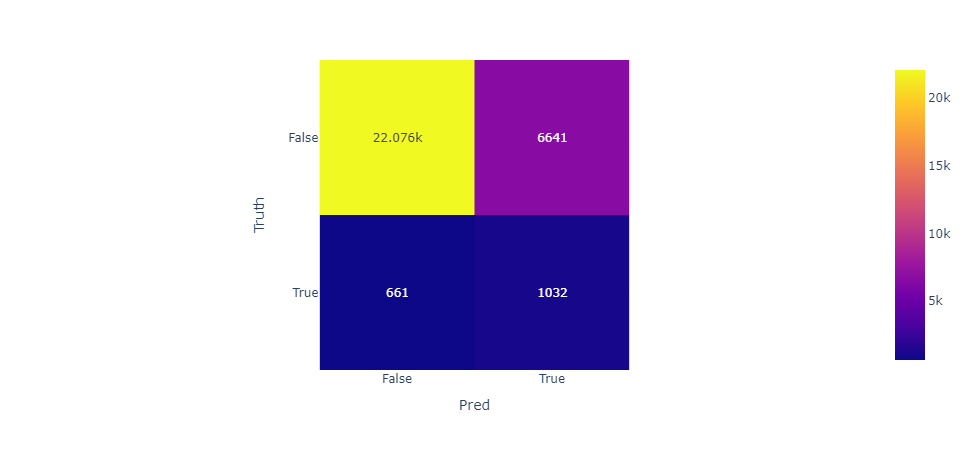
\includegraphics[width=8cm]{./img/DIR_confusion_matrix.png}
            \caption{Matrice de confusion avec Disparate Impact Remover}\label{fig:DIR_matrix}
        \end{subfigure}
        \hspace{0.2cm}
        \begin{subfigure}{6cm}
            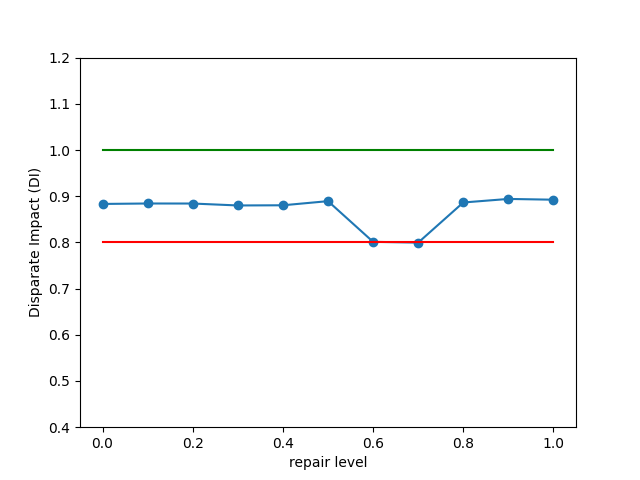
\includegraphics[width=6cm]{./img/disparate_impact_remover.png}
        \caption{Disparate impact en fonction du paramètre \textit{level}}\label{fig:DIR_param}
        \end{subfigure}
        \caption{Résultats disparate impact remover}\label{fig:DIR}
    \end{figure}
    

    \section{In-processing}

    \subsection{Adversarial debiasing}
    \subsubsection{Explications}
    Cette méthode vise à entrainer un classifieur pour maximiser l'accuracy tout en réduisant la possibilité pour un second 
    modèle de prédire la sortie en fonction de l'attribut sensible. En réduisant la possibilité de prédire la sortie en 
    fonction de l'attribut sensible, on réduit les biais sur cet attribut.
    La spécificité de cette méthode par rapport aux autres est donc qu'elle n'utilise plus le modèle que nous avons 
    défini auparavant mais un autre modèle.

    \subsubsection{Résultats}
    Les résultats obtenus sont plutôt intéressants que ce soit sans ou avec la réduction de biais. En effet, on remarque que 
    dans les deux cas le disparate impact est supérieur à 1. Nous pouvons expliquer cela par le fait 
    que cette méthode n'utilise pas de \texttt{RandomForestClassifier}, ce qui donne des résultats très différents. 
    L'accuracy dimunue légèrement avec la réduction des biais mais reste aux alentours de $0.80$. On note que l'accuracy 
    sans réduction des biais est elle moins élevée qu'avec notre modèle. La figure~\ref{fig:ADV_matrix1} nous montre les 
    résultats obtenus avec ce modèle. Nous pouvons remarquer que le nombre de prédictions vraies est plutôt 
    intéressant mais plus faible que le nombre de prédictions faussements négatives. 
    
    Les résultats obtenus avec cette méthode sont tout de même très intéressants car nous conservons une accuracy 
    acceptable tout en ayant un très bon disarate impact. En revanche, l'objectif étant d'améliorer notre modèle 
    (une forêt aléatoire) en réduisant ses biais, l'utilisation d'un nouveau modèle que nous connaissons peu 
    est discutable.

    \subsubsection{Un peu de pre-processing}
    Les résultats obtenus avec ce modèle sont intéressants c'est pourquoi nous avons voulu ajouter 
    du pre-processing afin d'essayer de l'améliorer d'avantage et notamment au niveau de l'accuracy.
    Nous avons choisi d'utiliser la repondération qui a donné d'excellents résultats sur notre 
    modèle utilisant une forêt aléatoire.
    Les résultats obtenus sont meilleurs que sans repondération. Sur la matrice de confusion 
    figure~\ref{fig:ADV_matrix2} on peut voir que les vrais positifs ont légèrement diminués. 
    Cependant on remarque que le nombre de faux positifs a fortement diminué au 
    profit des vrais négatifs. 
    
    On obtient avec ce modèle des métriques de fairness aussi bonne qu'avant avec un disparate impact 
    légèrement supérieur à 1, une equal opportunity difference proche de 0 tout en ne diminuant pas 
    l'accuracy qui est maintenant de $0.83$.


    \begin{figure}[h]
        \centering
        \begin{subfigure}{7cm}
            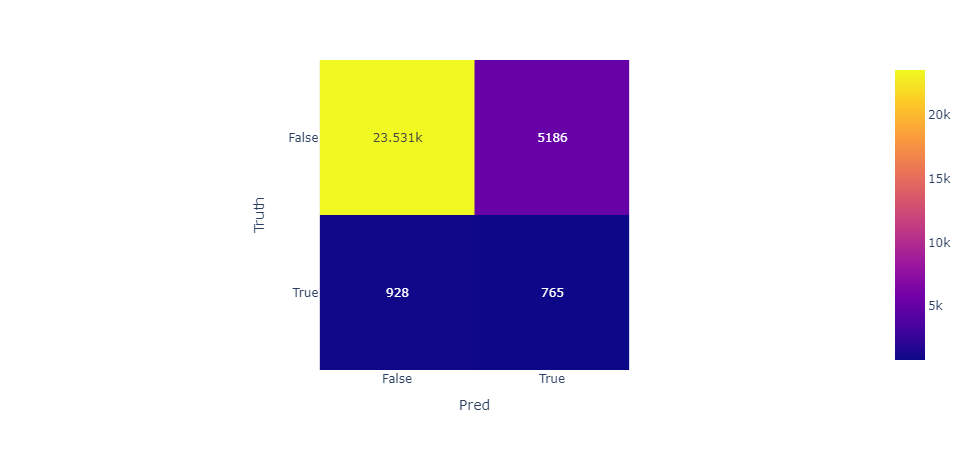
\includegraphics[width=7cm]{./img/adversarial1_conf_matrix.png}
            \caption{Sans pre-processing}\label{fig:ADV_matrix1}
        \end{subfigure}
        \hspace{0.2cm}
        \begin{subfigure}{7cm}
            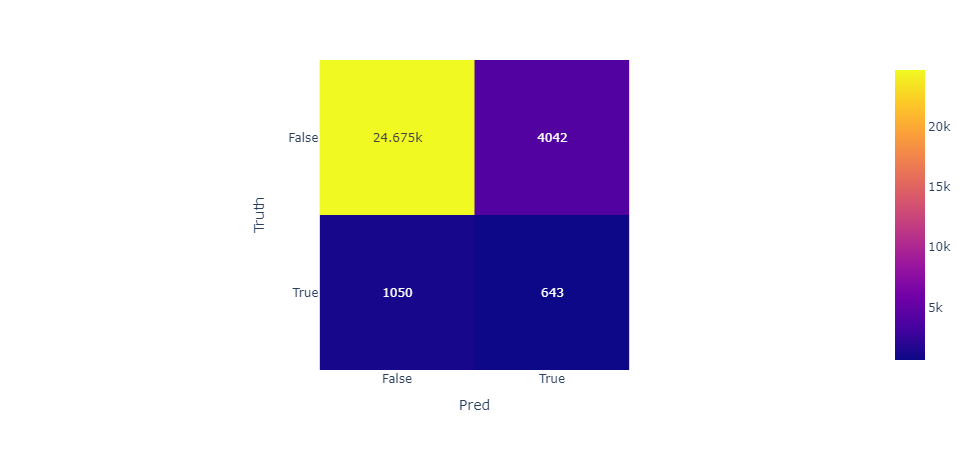
\includegraphics[width=7cm]{./img/adversarial2_conf_matrix.png}
        \caption{Avec repondération des données}\label{fig:ADV_matrix2}
        \end{subfigure}
        \caption{Matrices de confusions de modèles Adversarial debiasing avec réduction de biais}
    \end{figure}


    \section{Post-processing}

    \subsection{Reject option classification}
    \subsubsection{Un nouveau seuil}

    Le but de cette méthode de correction de biais post-preprocessing, est de faire varier le seuil de décision de manière à 
    trouver celui qui a la meilleure fairness, pour le comparer au seuil ayant la meilleure accuracy.

    Toujours à l'aide d'AIF 360, nous avons utilisé ROC en paramétrant le groupe privilégié à 1 (Hommes) et les lésés à 0 (Femmes).
    Les résultats sont les seuils suivant: 

    \begin{itemize}
        \item Sans fairness : \textit{0.1189}
        \item Avec fairness : \textit{0.1289}
    \end{itemize}
    
    De ces résultats on peut sortir deux observations. Tout d'abord, ROC a trouvé qu'il faudrait déplacer le seuil de sorte à corriger 
    un biais. Ensuite, la correction effectuée est minime dans son ampleur. 

    \subsubsection{Les nouvelles performances du modèle}

    Les répercussions sur l'accuracy sont quant à elles plus que notables. On passe en effet de \textit{0,876} à \textit{0,640}.
    Cependant, si on regarde un peu plus en détail la matrice de confusion, il parrait intéressant de noter que ce modèle détecte mieux 
    les accidents mortels véritablement mortels. Pour être précis,on détecte \textit{79\%} des accidents
    mortels répertoriés dans l'ensemble (rappelons que les scores et la matrices sont ici calculés sur le set de validation qui est deux fois plus petit en effectifs). 
    Ceci se fait au prix d'un augmentation des accidents non mortels faussement détectés. Malgré tout, 
    le taux de détection de ce type d'accident reste assez élevé à \textit{63\%}. En définitive, il catégorise trop de véhicules comme causant des accidents mortels.
    Cela fait que ce modèle est bien moins fiable. Mais il a l'intêret, que lorsqu'un véhicule n'est pas classifié comme mortellement accidenté, 
    on peut être très confiant sur cette prédiction. 

    \subsubsection{Les performances pour la fairness}

    La première observation que l'on peut faire, c'est que le disparate impact se voit corrigé. Pour être précis, avec le nouveau seuil, le disparate impact
    augmente à \textit{0.98}. On peut donc voir ici que le disparate impact homme / femme est presque rectifié. 
    
    On remarque aussi que les taux d'erreurs 
    \[ P(\overline{Y}=1| (Y=1, Z=0)) \] \[ P(\overline{Y}=1| (Y=0, Z=0)) \] \[ P(\overline{Y}=1| (Y=1, Z=1)) \] \[ P(\overline{Y}=1| (Y=0, Z=1)) \] chez les femmes se sont rapprochés de
    ceux des hommes. Cela atteste d'une correction de biais substentielle.  

    En revanche, il faut souligner que la correction de biais n'est pas parfaite. On peut même dire qu'elle est très légèrement inférieure à d'autres méthodes telles que reweighing.
    
    \subsection{Calibrated equalized odds}
    \subsubsection{Explications}
    Cette méthode modifie les sorties du modèle afin d'augmenter l'égalité entre les valeurs de l'attribut 
    sensible. Cette méthode est testée sur différents seuils de prédiction afin de trouver le modèle le plus efficace.
    On note cependant que les résultats son assez dépendants de l'aléatoire. Ils 
    peuvent être variables d'une exécution à l'autre et peuvent même donner de moins bons résultats que sans le 
    post-processing, ce nous allons voir par la suite.

    \subsubsection{Les résultats obtenus}
    La figure~\ref{fig:EQU_odds} nous montre l'évolution de l'accuracy et de l'égalité de l'attribut sensible 
    (ici homme/femme) dans les prédictions en fonction du seuil. L'objectif est d'avoir l'accuracy la plus élevée tout 
    en ayant le plus d'égalité sur l'attribut sensible (donc \textit{equal opportunity difference} le plus proche de 0).
    Le résultat obtenu nous montre que l'application de cette méthode a ici eu un effet négatif. En effet nous pouvons 
    remarquer que le meilleur résultat obtenu est avant post-processing avec un seuil légèrement en dessous de $0.15$.
    Comme dit précédemment, les résultats varient avec l'aléatoire et on arrive à avoir des cas où les résultats sont 
    meilleurs avec le post-processing.

    

    \subsubsection{Mise en perspective}
    Comme nous avons pu le voir ce résultat n'est pas vraiment satisfaisant. Cependant cette méthode reste très
    intéressante pour avoir une vu globale du modèle et des résultats obtenus.
    Le \texttt{RejectOptionClassifier} vu précédemment nous indique directement un seuil optimal sans qu'on ait 
    une idée de comment évoluent les biais en fonction du seuil. Ici nous avons des résultats selon les 
    différents seuils. De plus une donnée intéressante ici est la visulisation de l'accuracy. Cela 
    nous permet de réduire les biais tout en ayant le contrôle de l'accuracy (que ce soit avec ou sans 
    post-processing), ce qui n'est pas forcément évident avec les autres méthodes.
    
    \begin{figure}[h]
        \centering
        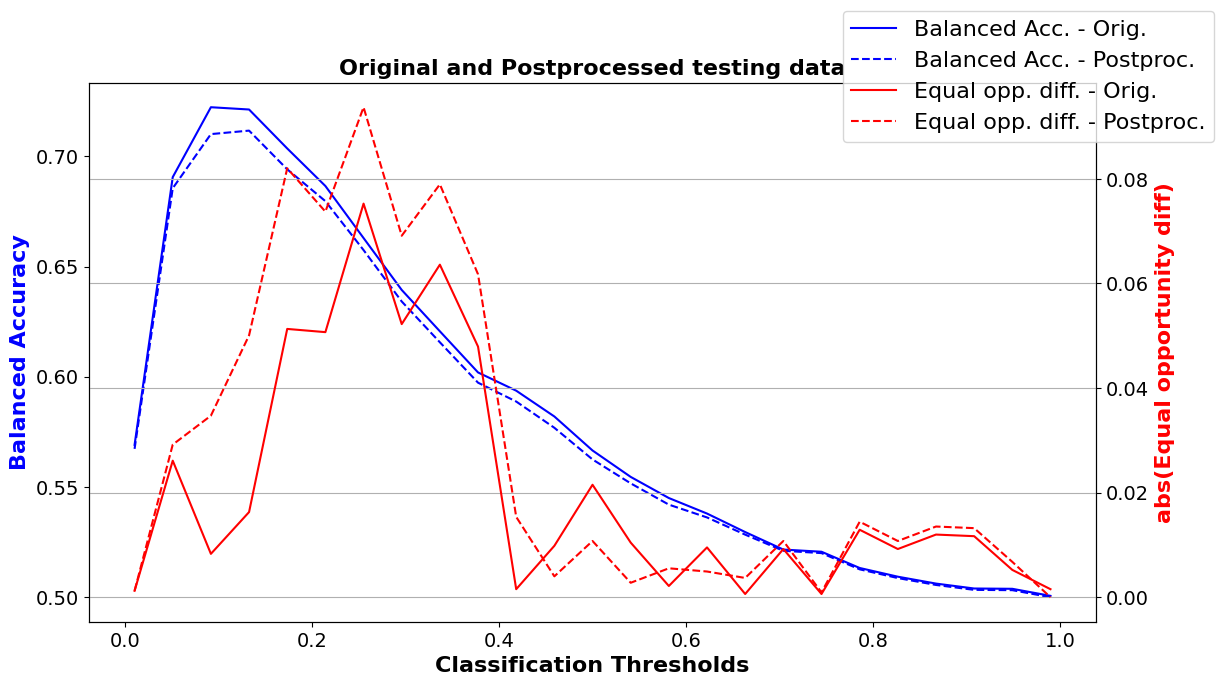
\includegraphics[width=\textwidth]{./img/cal_equ_odds.png}
        \caption{Résultats avec et sans post-processing en fonction du seuil}
        \label{fig:EQU_odds}
    \end{figure}
    \vspace{3cm}

    \newpage
    \section{Conclusion}

    \subsection{Les résultats obtenus}
    À la fin de la première partie de ce projet (développement d'un modèle et analyse) nous avions pu 
    identifier le sexe du conducteur comme un attribut sensible de notre dataset. Ce premier modèle 
    sans correction des biais obtenait une accuracy de $0.87$. Malgré ce score plutôt acceptable, nous 
    avions pu remarquer que les bonnes prédictions de la classe \textit{mortel} étaient moins fréquentes et 
    que la grande quantité de données de la classe \textit{non mortel} contribuait fortement à ce score. 
    Le défit dans cette seconde partie a été de réduire le plus possible les biais de notre modèle, tout 
    en essayant de conserver un modèle le plus efficace possible. Nous pensons avoir plutôt bien relevé ce 
    défis avec le travail effectué.

    Si on observe globalement les méthodes utilisées, on peut remarquer que pour la plupart elles 
    diminuent le disparate impact de notre modèle à un niveau acceptable (au-dessus de 0.80). De même lorsqu'on 
    observe l'\textit{equal oppotunity difference}, la valeur est bien réduite. 
    Nous avons cependant noté trois méthodes qui ont particulièrement attirées notre attention.

    Premièrement, nous avons la repondération (reweighing). La repondération de notre jeu de données a 
    permis de réduire grandement les biais du modèle. De plus contrairement aux autres méthodes de 
    pre-processing elle a l'avantage d'être rapide et facilement adaptable à notre modèle utilisant une 
    pipeline. Enfin, cette méthode réduit l'accuracy du modèle mais en observant la matrice de confusion 
    on remarque que les prédictions de la classe \textit{mortel} sont plus élevées que les faux négatifs, 
    ce qui n'était pas le cas précédemment et qui peut paraitre préférable.

    Ensuite, les résultats de l'adversarial debiasing sont parmis les plus concluants. En effet cette 
    méthode permet d'obtenir un modèle plutôt efficace tout en ayant d'excellentes métriques de fairness avec 
    par exemple un disparate impact proche de 1. Comme expliqué dans la section dédiée, ce modèle reste cependant 
    un modèle plus éloigné du travail effectué précédemment car il met de côté notre modèle. Nous pensons par
     conséquent qu'il est important d'étudier les alternatives qui peuvent s'adapter à notre propre modèle.
    C'est pour nous une manière d'avoir plus de contrôle sur le modèle.

    Enfin, la dernière méthode que nous avons trouvé intéressante est la reject option classification. On 
    obtient encore une fois d'excellents résultats aux niveaux des métriques avec également l'un des balanced 
    accuracy les plus élevés. On a pu remarquer ces bons résultats sur la matrice de confusion associée.

    \subsection{Aller plus loin}
    Nous avons pu remarquer lors de l'analyse des données que d'autres attributs sont des sources de biais pour 
    notre modèle. Il serait intéressant de poursuivre la correction des biais avec ces attributs 
    sensibles. Nous pouvons par exemple penser aux attributs \textit{âge} ou \textit{mois}. 
    
    Ce projet a pour objectif de travailler sur la fairness en IA. Aller plus loin pourrait également 
    signifier dépasser cet objectif et améliorer le modèle afin d'obtenir d'en tirer de meilleures 
    performances (tout en conservant un modèle le moins biaisé possible).

    \subsection{Un projet enrichissant}
    Le travail effectué au cours de ce projet a été très enrichissant pour nous. Il nous a permis de 
    découvrir un aspect plus humain de l'intelligence artificielle. Il est effectivement important de 
    conprendre que les modèles sont dépendants des données qu'on leur fournit et que ces données ne 
    sont pas parfaites. Le modèle sur lequel nous avons pu travailler ici a probablement peu d'utilité 
    dans le monde réel mais il fait prendre conscience des problèmes auxquels on peut faire face.
    Nous avions jusqu'ici appris à préparer des données pour l'apprentissage, réaliser l'apprentissage et
    évaluer les performances sans jamais faire attention aux biais et aux problèmes qui peuvent en découler.
    Il ne fait aucun doute qu'après le travail effectué avec ce cours cette question aura une place 
    importante lorsque nous parlerons d'apprentissage machine.


    \newpage
    \appendix

    \section{Les données conservées pour le modèle.}\label{appendix:dataset}
    \begin{center}
        \begin{tabular}{ |c|p{9cm}| }
            \hline
            \textbf{Attribut} & \textbf{Description} \\
            \hline
            \textit{Num\_Acc} & Numéro d'identifiant de l'accident \\
            \textit{jour mois} & Jour de l'accident, mois de l'accident \\
            \textit{an} & Année de l'accident \\
            \textit{hrmn} & Heure et minutes de l'accident \\
            \textit{lum} & Conditions d'éclairage dans lesquelles l'accident s'est produit \\
            \textit{dep} & Code INSEE du département \\
            \textit{agg} & Localisation en agglomération \\
            \textit{int} & Type d'intersection \\
            \textit{atm} & Conditions atmosphériques \\
            \textit{col} & Type de collision \\
            \textit{adr} & Adresse postale (pour les accidents en agglomération) \\
            \textit{lat} & Latitude \\
            \textit{long} & Longitude \\
            \textit{catr} & Catégorie de route \\
            \textit{voie} & Numéro de la route \\
            \textit{circ} & Régime de circulation \\
            \textit{nbv} & Nombre total de voies de circulation \\
            \textit{vosp} & Présence d'une voie réservée \\
            \textit{prof} & Profil en long de la route \\
            \textit{plan} & Tracé en plan de la route \\
            \textit{surf} & État de la surface de la route \\
            \textit{infra} & Présence d'aménagements ou d'infrastructures \\
            \textit{situ} & Situation géographique de l'accident \\
            \textit{vma} & Vitesses maximale autorisées \\
            \textit{id\_vehicule} & Identifiant du véhicule (clé étrangère) \\
            \textit{catv} & Catégorie du véhicule impliqué dans l'accident \\
            \textit{obs} & Type d'obstacle heurté \\
            \textit{obsm} & Type d'obstacle mobile heurté \\
            \textit{choc} & Point de choc initial \\
            \textit{manv} & Manœuvre principale avant l'accident \\
            \textit{catu} & Catégorie d'usager (conducteur, passager, piéton) \\
            \textit{grav} & Gravité de l'accident pour l'usager \\
            \textit{sexe} & Sexe du conducteur \\
            \textit{trajet} & Motif du déplacement au moment de l'accident \\
            \textit{mortal} & Indique si le véhicule est impliqué dans un accident mortel (calculé dans le notebook) \\
            \hline
        \end{tabular}
    \end{center}
    \newpage

    \section{Les données abandonnées et la raison de leur abandon}\label{appendix:dataset}
    \begin{center}
        \scriptsize
        \begin{tabular}{ |c|p{3.5cm}|p{7cm}| }
            \hline
            \textbf{Attribut} & \textbf{Description} & \textbf{Raison de l'abandon} \\
            \hline
            \textit{id\_vehicule} & Identifiant numérique unique du véhicule & information administrative, une fois les tables jointes, cette information sans intéret, n'est plus utile\\
            \textit{num\_veh} & Identifiant du véhicule pour associer les passagers du même vehicule & Information administrative, une fois les tables jointes, cette inforamtion sans intêret, n'est plus utile\\
            \textit{id\_usager} & Identifiant des usagers dans la base & Utilisé lors des jointures, inutile par la suite\\
            \textit{com} & Numéro de commune (code INSEE) & Commune trop spécifique, ça donne trop de catégories\\
            \textit{adr} & Adresse de l'accident & Trop spécifique, ne donne rien de pertinent\\
            \textit{lat} & Latitude de l'accident & Ces informations positionelles ne reflètent pas le type d'endroit où l'accident a lieu\\
            \textit{Long} & Longitude de l'accident & Ces informations positionelles ne reflètent pas le type d'endroit où l'accident a lieu\\
            \textit{Num\_Acc} & Numéro d'identifiant de l'accident & Information administrative, une fois les tables jointes, cette inforamtion sans intêret, n'est plus utile\\
            \textit{voie} & Numéro de la route & Pas pertinent, plusieurs routes ont le même numéro, certaines routes ont des sections plus dangereuses que d'autres\\
            \textit{V1} & Numéro de la route & Pas pertinent, plusieurs routes ont le même numéro, certaines routes ont des sections plus dangereuses que d'autres\\
            \textit{V2} & Numéro de la route & Pas pertinent, plusieurs routes ont le même numéro, certaines routes ont des sections plus dangereuses que d'autres\\
            \textit{vosp} & Signale l'existence d'une voie réservée, indépendamment du fait que l'accident ait eu lieu ou non sur cette voie. & Attribut trop peu renseigné, peu d'accidents concernés\\
            \textit{pr} & Numéro de la borne (routière) en amont  & Pas pertinent, beaucoup de routes sont non bornées, n'indique rien d'intéressant sur l'accident\\
            \textit{pr1} & Distance en mètres à la borne en amont &  Pas pertinent, beaucoup de routes sont non bornées, n'indique rien d'intéressant sur l'accident\\
            \textit{lartpc} & Largeur terplein central en mètres & Trop peu renseigné\\
            \textit{larrout} & Largeur de la chaussée en mètres & Trop peu renseigné\\
            \textit{senc} & Indique si le véhicule allait vers une borne supérieure ou inférieure à la précédente. & Information administrative, pas utile\\
            \textit{manv} & Indique la manoeuvre en cours au moment de l'accident & Trop souvent inconnue ou non renseignée\\
            \textit{motor} & Motorisation du véhicule & Trop peu renseignée\\
            \textit{place} & Place du passager dans l'habitacle, 10 indique un piéton & Utilisée pour trouver les conducteurs et les piétons, devient inutile à l'échelle de l'accident ensuite\\
            \textit{grav} & Donne l'état de gravité de l'usager accidenté & Utilisée pour trouver les accidents mortels, devient inutile à l'échelle de l'accident ensuite\\
            \textit{sexe} & Sexe de l'usager (binaire) & Utilisé pour déterminer le sexe du conducteur, devient inutile à l'échelle de l'accident ensuite\\
            \textit{secu1, secu2, secu3} & Trois attributs renseignant tous les 3 sur l'utilisation d'équipements de sécurité & Attribut difficilement implémentable et peu fiable car non renseigné apparait beaucoup\\
            \textit{locp} & Localisation du piéton par rapport au véhicule & Le point de vue de l'accident rend difficile l'implémentation de cet attribut peu renseigné\\
            \textit{actp} & Action piéton lors de l'accident & Le point de vue de l'accident rend difficile l'implémentation de cet attribut peu renseigné\\
            \textit{etatp} & Précise si le pieton était accompagné & Le point de vue de l'accident rend difficile l'implémentation de cet attribut peu renseigné\\
            \textit{occutc} & Nombre d'occupants du transport en commun & Cet attribut est trop peu renseigné\\
            \textit{jour} & Numéro du jour de l'accident & Peu utile, il aurait été plus utile de connaitre le jour de la semaine\\
            \textit{hrmn} & Heures : minutes & Format non adapté, redondant de luminosité (lum) qui est plus précis\\
            \textit{an} & Année de l'accident & Utilisée pour déterminer l'âge du conducteur, n'est plus utile par la suite \\
            \textit{an\_nais} & Année de naissance de l'usager & Utilisée pour déterminer l'âge du conducteur, n'est plus utile par la suite, pas adapté au point de vue de l'accident \\
            \hline
        \end{tabular}
    \end{center}
    \newpage

    \section{Diagrammes en cascade des valeurs de Shapley}
    \begin{figure}[ht]
        \centering
        \begin{subfigure}{9cm}
            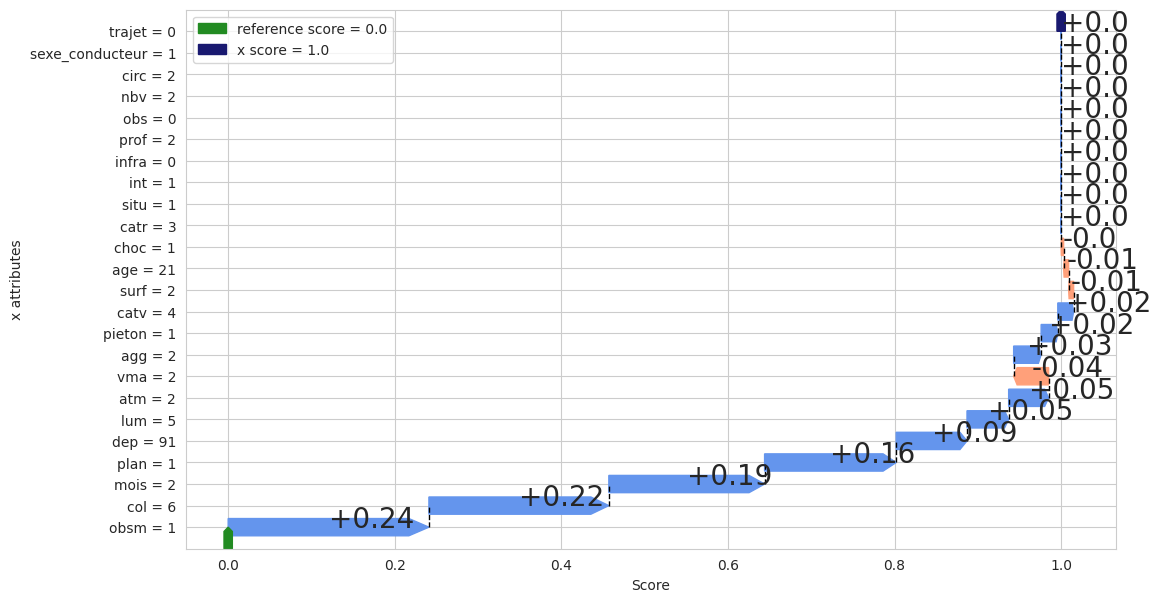
\includegraphics[width=9cm]{./img/shap10.png}
            \caption{}
        \end{subfigure}
        \begin{subfigure}{9cm}
            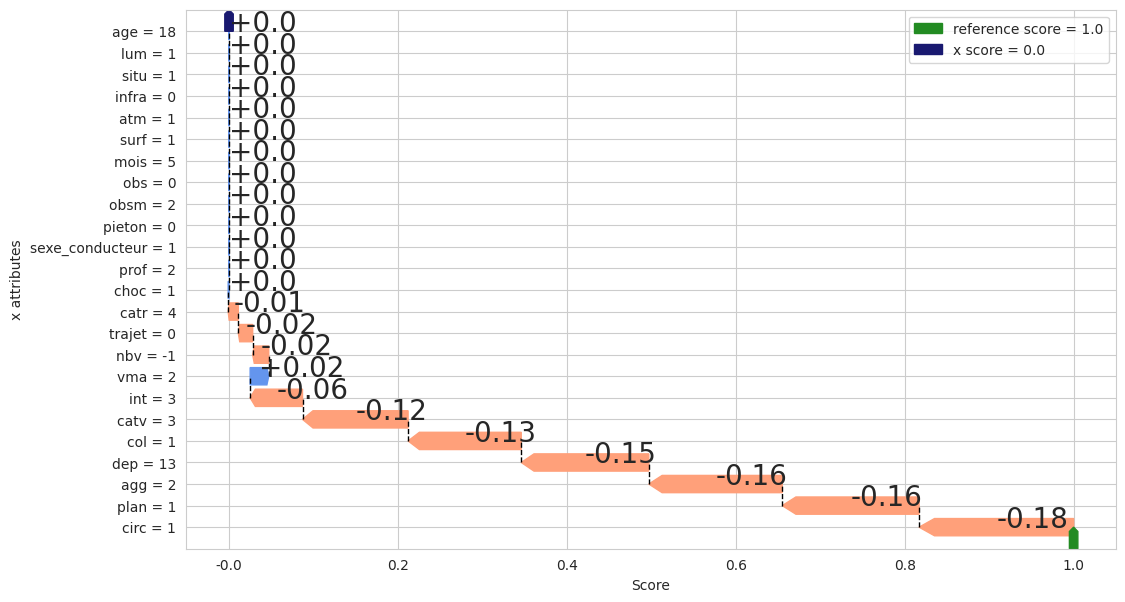
\includegraphics[width=9cm]{./img/shap8.png}
        \caption{}
        \end{subfigure}
        \begin{subfigure}{9cm}
            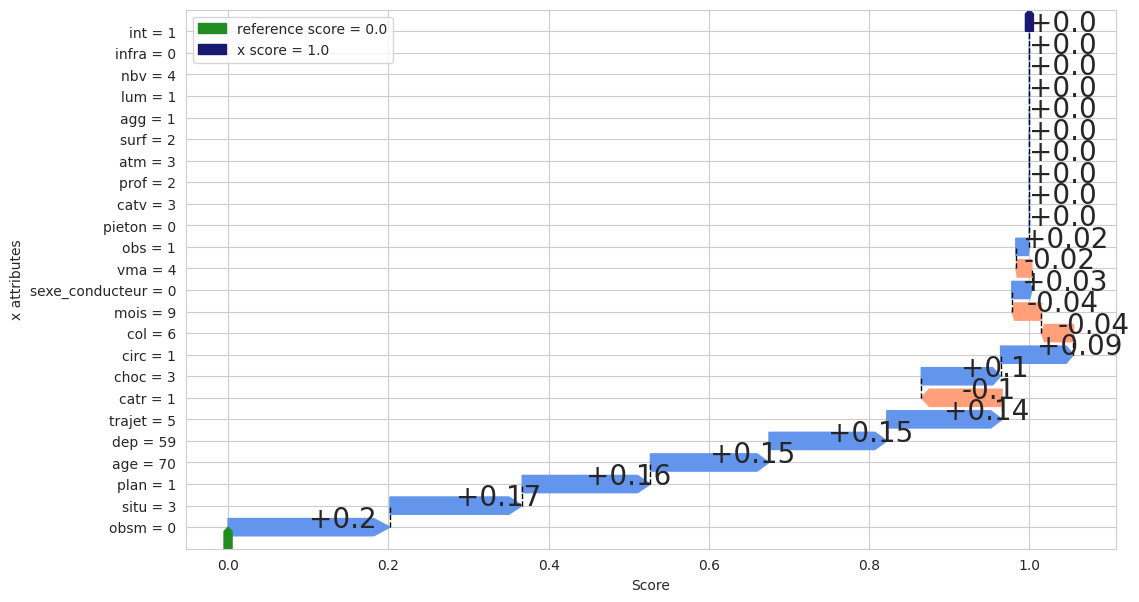
\includegraphics[width=9cm]{./img/shap9.png}
        \caption{}
        \end{subfigure}
    \end{figure}
    \begin{figure}[ht]
        \centering
        \begin{subfigure}{9cm}
            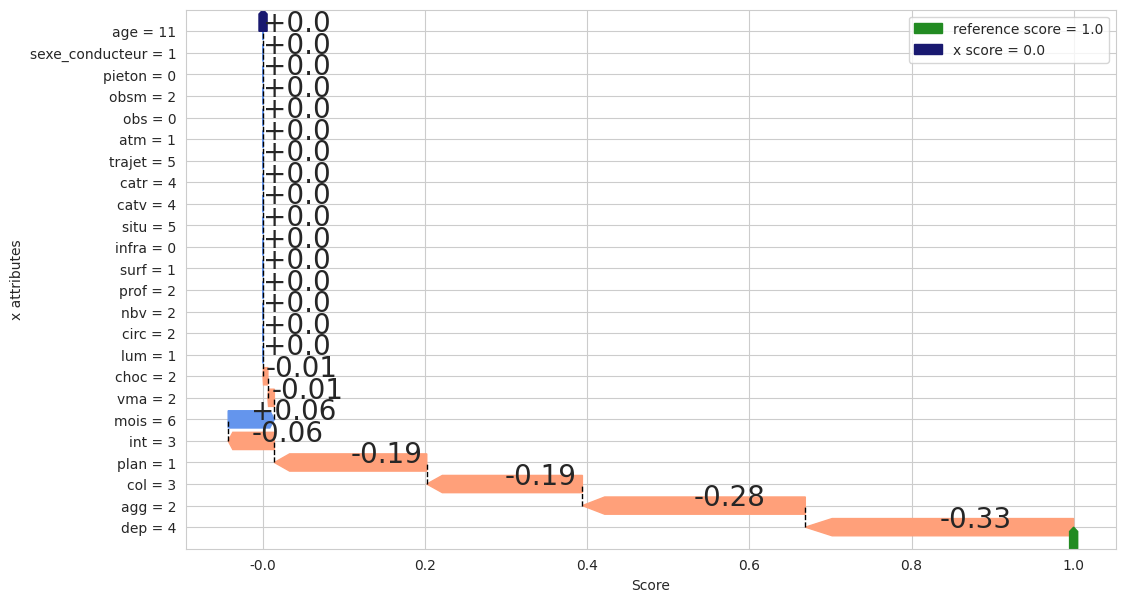
\includegraphics[width=9cm]{./img/shap7.png}
            \caption{}
        \end{subfigure}
        \begin{subfigure}{9cm}
            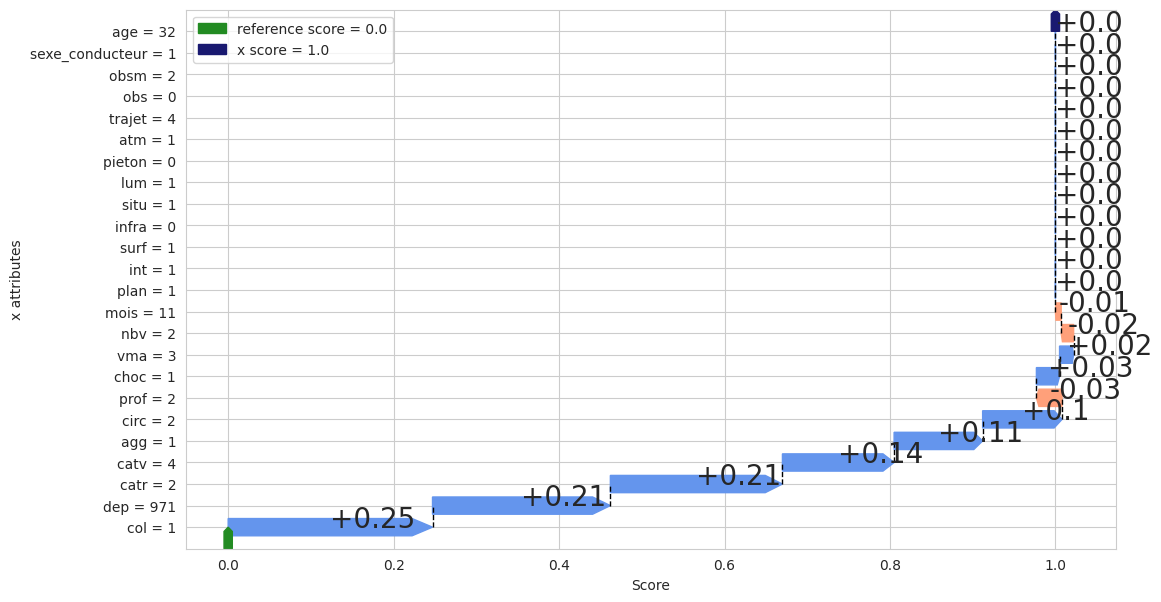
\includegraphics[width=9cm]{./img/shap6.png}
        \caption{}
        \end{subfigure}
        \begin{subfigure}{9cm}
            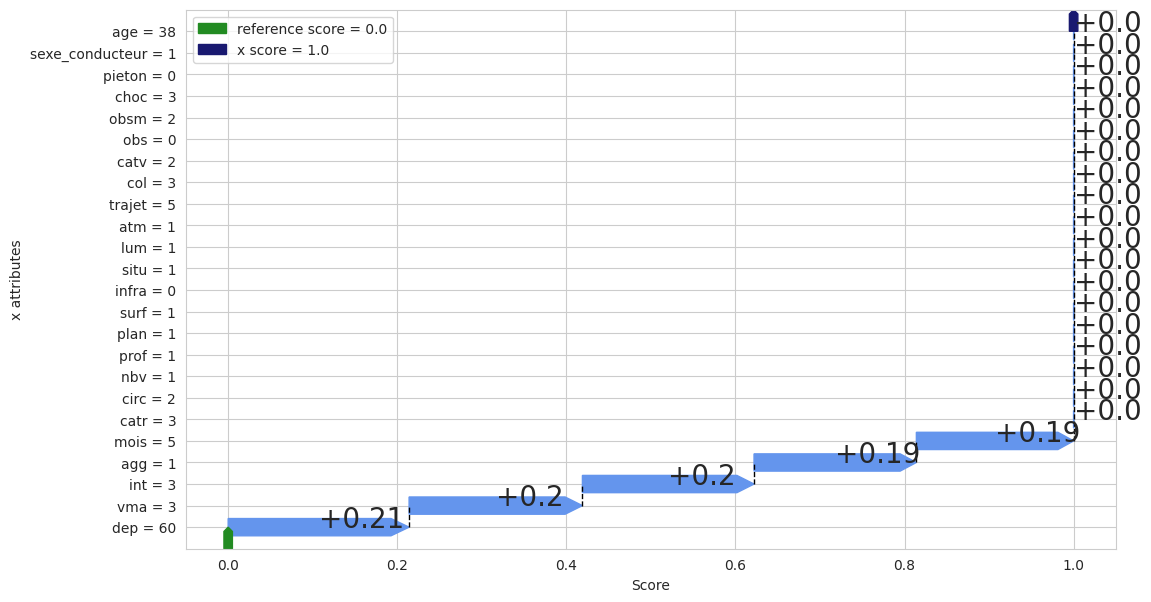
\includegraphics[width=9cm]{./img/shap5.png}
        \caption{}
        \end{subfigure}
    \end{figure}

\end{document}